\documentclass[11pt]{article}
\usepackage[T1]{fontenc}
\usepackage[utf8]{inputenc}
\usepackage{lmodern}
\usepackage{amsmath,amssymb,amsthm,mathtools}
\usepackage[margin=1in]{geometry}
\usepackage{microtype,booktabs,longtable,array,enumitem,xcolor}
\usepackage{graphicx,listings,fancyhdr}
\usepackage[hidelinks]{hyperref}
\usepackage{xurl}
\hypersetup{pdftitle={Finite algebra and stable selection in iPRA},pdfauthor={Research report prepared for Vladimir Reshetnikov}}
\newcommand{\ipra}{\mathsf{iPRA}}
\newcommand{\N}{\mathbb N}
\newcommand{\Z}{\mathbb Z}
\newcommand{\Q}{\mathbb Q}
\newcommand{\R}{\mathbb R}
\newcommand{\C}{\mathbb C}
\newcommand{\Norm}{\operatorname{N}}
\newcommand{\ord}{\operatorname{ord}}
\newcommand{\lc}{\operatorname{lc}}
\newcommand{\Span}{\operatorname{span}}
\newcommand{\sgn}{\operatorname{sgn}}
\newcommand{\dist}{\operatorname{dist}}
\newcommand{\PR}{\mathsf{PR}}
\newcommand{\code}[1]{\texttt{\small #1}}
\newcommand{\pin}{3ee850b4c2d650cf01263823fd5415963747c5d0}
\newtheorem{theorem}{Theorem}[section]
\newtheorem{lemma}[theorem]{Lemma}
\newtheorem{proposition}[theorem]{Proposition}
\newtheorem{corollary}[theorem]{Corollary}
\theoremstyle{definition}
\newtheorem{definition}[theorem]{Definition}
\newtheorem{example}[theorem]{Example}
\newtheorem{remark}[theorem]{Remark}
\newtheorem{contract}[theorem]{Contract}
\setlist{itemsep=3pt,topsep=5pt}
\setlength{\emergencystretch}{2em}
\newcolumntype{P}[1]{>{\raggedright\arraybackslash}p{#1}}
\setlength{\headheight}{14pt}
\pagestyle{fancy}
\fancyhf{}
\fancyhead[L]{\small Finite algebra and stable selection in $\ipra$}
\fancyhead[R]{\small 19 November 2026}
\fancyfoot[C]{\thepage}
\lstset{basicstyle=\ttfamily\footnotesize,breaklines=true,columns=fullflexible,keepspaces=true,frame=single,rulecolor=\color{black!20}}
\begin{document}
\hypersetup{pageanchor=false}
\begin{titlepage}
\vspace*{1cm}
\begin{center}
{\Large\bfseries Finite algebra and stable selection in $\ipra$\par}
\vspace{0.4cm}
{\large A general embedding discipline with two concrete extensions\par}
\vspace{0.7cm}
Prepared for Vladimir Reshetnikov\\[4pt]
19 November 2026
\end{center}
\vspace{0.7cm}
\begin{abstract}
We develop a framework for translating mathematical constructions into intuitionistic primitive recursive arithmetic by separating finite representations, actual primitive recursive producers, bounded correctness invariants, and external semantic interpretation. The framework reuses the current ProveIt arithmetic and finite-observation infrastructure rather than replacing it.

The main algebraic extension separates a bound on a determinant norm from its nonvanishing proof. Repeated polynomial division and a reduced quotient algebra prove automatic nonvanishing for $y^m=f(x)$ whenever the nonconstant rational polynomial $f$ is squarefree, with no coprimality restriction on the global degrees. A more general divisor certificate covers some repeated-factor inputs. A local Newton certificate also handles mixed equations. These results yield explicit finite common-zero and proper-subspace bounds. We additionally compress the existing leading-form test from dimension $m$ to $\gcd(m,d)$.

The complementary analytic construction selects a canonical point from finite Hausdorff approximations to a nonempty compact convex set. Finite least-square minimization, approximate midpoint convexity, and a quantitative cancellation estimate produce a fast Cauchy name without an exact minimum value or a preselected limiting witness.

All main arguments are developed at the human mathematical level, with explicit algorithms and induction obligations. The archive supplies exact-arithmetic experiments, a current-source audit, Lean candidate code, and detailed object-theory blueprints. New Lean files were not kernel-checked in this environment. Existing checked upstream declarations are clearly distinguished from the new results and from external completion semantics. No general Siegel, Faltings, or unrestricted selection theorem is claimed.
\end{abstract}
\vfill
\noindent\textbf{Source snapshot.}\quad ProveIt main, commit\\
\texttt{\pin}.\\[6pt]
\textbf{Verification boundary.}\quad Human proofs and exact finite computations; explicit Lean completion plan. Upstream proof status is reported from the pinned source, not from a new full repository build.
\end{titlepage}
\hypersetup{pageanchor=true}
\pagenumbering{roman}
\tableofcontents
\clearpage
\pagenumbering{arabic}
\section{What the present work adds}
\label{sec:scope}

The requested task is not merely to encode the vocabulary of analysis or algebra in arithmetic. A useful embedding must preserve the requested mathematical conclusion, give the actual finite constructions used to obtain it, and expose the induction needed to justify them. An algorithm that checks a proposed solution is not yet an algorithm that produces one. A Lean theorem about the standard natural numbers is not yet an object-theory derivation in $\ipra$.

Those distinctions are already central to the ProveIt project. The current repository has also progressed considerably beyond its archived research packets. Its source-level audit records complete implementations of fixed-syntax bounded Booleanization, backward demand transfer, parameter-changing recursion, finite-query induction, finite Hausdorff operations, actual approximate-root programs, and concrete monic root-support constructions \cite{repo-audit,repo-derivations}. Reproposing those as missing infrastructure would misidentify the present problem.

Our contribution has three parts. First, we organize the shared embedding discipline around an explicit boundary between a fixed program schema and its internal numerical inputs. Second, we develop new certificate producers and strengthened algebraic hypotheses that address an actually open norm endpoint. Third, we give a canonical selection construction that works on nonunique convex solution sets while retaining an explicit finite approximation requirement.

\subsection{A source-sensitive status table}

\begin{longtable}{@{}P{0.23\textwidth}P{0.34\textwidth}P{0.37\textwidth}@{}}
\toprule
Topic & Pinned source status & Treatment here\\
\midrule
\endhead
Bounded formulas & The fixed grammar has actual object-theory compilation and reflection. & Reuse it; do not introduce a universal evaluator for arbitrary program codes.\\[5pt]
Demand and changing precision & Predetermined backward-demand and two-pass recursion are already derived. & Use their local-contract discipline. No new general compiler is claimed.\\[5pt]
Rational norms & The runtime multiplication matrix, determinant, fields, and evaluation action have been constructed. & Supply mathematical degree, nonvanishing, fiber-multiplicity and annihilator arguments, plus exact links to remaining object endpoints.\\[5pt]
Coprime weighted zero counts & Human arguments exist; the source audit still leaves the full runtime norm endpoint open. & Reprove the common-zero mechanism for completeness, credit the existing result, and extend it using finite-place certificates.\\[5pt]
Initial-form norm test & Already present in the coherent-methods packet, including some noncoprime cases. & Credit this general test. The smaller $\gcd(m,d)$ determinant is an additional simplification.\\[5pt]
Strong minimizers & Existing derivations use finite minimization and strong convexity with explicit adapters. & Remove the need for a supplied exact baseline value in the key comparison, then construct a canonical convex-set selector from actual finite lists.\\[5pt]
Siegel/Faltings & General effective covers and/or height producers are not supplied by the inspected packets. & Retain these as explicit boundaries; a better zero count does not produce a global cover or a height bound.\\
\bottomrule
\end{longtable}

Here and below, ``new'' means a development relative to the sources audited in this task. We make no claim that these elementary valuation and projection ideas are new to mathematics. The point is a precise, reusable route into the project's restricted arithmetic, with the necessary data made explicit.

\subsection{The strongest algebraic conclusion}

Consider the reduced polynomial
\[
 G(X,Y)=\sum_{j<m}A_j(X)Y^j\ne0
\]
on $Y^m=f(X)$. Set
\[
 W(G)=\max_{A_j\ne0}\{m\deg A_j+d j\},\qquad d=\deg f.
\]
The earlier automatic argument uses $\gcd(m,d)=1$ to show that the determinant norm is nonzero and has degree exactly $W(G)$. We separate these conclusions. A global weight calculation gives the upper bound $\deg\Norm(G)\le W(G)$ without coprimality, whenever the norm is nonzero. A supplied finite point $a$ at which $f$ has positive order $e$ coprime to $m$ proves that nonvanishing independently.

In particular, $f=X^d+X$ has order one at zero when $d\ge2$. Thus every finite list of distinct common zeros of
\[
 y^m=x^d+x,\qquad G(x,y)=0
\]
has length at most $W(G)$, for \emph{every} $m,d\ge2$. No factorization or irreducibility decision is needed. An analogous local Newton certificate works for mixed monic equations, proved in Section~\ref{sec:local}.

This conclusion is deliberately a bound on a supplied finite list. A complete list of all rational or integral points requires additional information. The distinction is essential for a correct statement in first-order arithmetic.

A stronger automatic version applies to every nonconstant squarefree $f\in\Q[X]$. Repeatedly divide each nonzero $A_j$ by $f$ to write $A_j=f^{a_j}B_j$, with $B_j\bmod f\ne0$. The weights $ma_j+j$ have a unique minimum $s$, at an index $k$. The determinant has the exact form
\[
 \Norm_{Y^m-f}(G)=f^s\left((-1)^{k(m-1)}B_k^m+fQ\right).
\]
A polynomial Bezout certificate for $f,f'$ proves that $\Q[X]/(f)$ has no nonzero nilpotents. Hence the bracket residue is nonzero, proving norm nonvanishing without finding or choosing a root. Section~\ref{sec:squarefree} proves this and a more general divisor criterion in full. The final bounds apply to the original rational input data.

\subsection{The analytic conclusion and its input strength}

Suppose a fixed primitive recursive program supplies nonempty finite rational lists $S_n$ approximating a compact convex set at a certified dyadic Hausdorff rate. Choose from $S_n$ a point whose squared distance to a supplied rational anchor is least. These independently computed choices have an explicit cross-stage distance bound. Reindexing at roughly twice the requested precision gives a fast Cauchy name for the nearest point.

The finite formulation only requires finite cross-list cover and approximate-midpoint certificates. The compact set enters when interpreting those certificates in ordinary analysis. A negatively described closed convex set, without such finite Hausdorff information, is a weaker input and is not covered. Theorems about convex choice depend strongly on the representation \cite{leroux-pauly}; the present construction keeps that dependence visible.

\section{A general discipline for embedding mathematics}
\label{sec:framework}

\subsection{The exact target theory}

We use first-order intuitionistic logic with equality, numerical variables, zero and successor, and a function symbol for each \emph{fixed} primitive recursive definition. Its nonlogical axioms are the defining equations of these symbols, successor injectivity, the impossibility of a successor being zero, and quantifier-free induction. In schematic notation the latter is
\[
 \bigl(A(0,\vec p)\wedge
       \forall n\,[A(n,\vec p)\to A(n+1,\vec p)]\bigr)
       \to\forall n\,A(n,\vec p),
\]
where $A$ is quantifier-free. Arbitrary numerical parameters $\vec p$ are allowed. First-order quantifiers may appear in theorems and in hypotheses; it is the induction formula that is restricted. The actual repository judgment is \code{Prf PRAAx}, with syntax and translations provided by ConciseIPRA \cite{repo-concise,repo-derivations}.

The logical rules are the ordinary intuitionistic introduction and elimination rules for $\wedge,\vee,\to,\bot,\forall,\exists$, structural substitution and weakening, and equality substitution. Quantifier-free numerical tests are decidable because their fixed primitive recursive characteristic functions have correctness proofs. This does not authorize excluded middle for arbitrary unbounded formulas.

\subsection{Fixed schema versus internal data}

An algorithm such as polynomial multiplication is fixed once. Polynomial coefficient lists, list lengths, degrees, matrix sizes, bounds and precision requests are numerical inputs to that algorithm. The theorem must quantify over those inputs internally. By contrast, a completely arbitrary primitive recursive program supplied as a code is not automatically available as a total arithmetic function.

\begin{proposition}[No primitive recursive universal evaluator]
There is no total primitive recursive function $U(e,n)$ that evaluates every unary primitive recursive function from its code in an enumeration containing every such function.
\end{proposition}
\begin{proof}
If $U$ existed, $D(n)=U(n,n)+1$ would be primitive recursive. Choose a code $e$ for $D$. Then $D(e)=U(e,e)+1=D(e)+1$, a contradiction. The argument concerns a total evaluator on all codes. Bounded simulation of programs for a supplied number of steps is a different, primitive recursive operation.
\end{proof}

Accordingly, a name $q(n,p)$ for a real number means one fixed primitive recursive rational-valued program with internal precision $n$ and persistent data $p$. A family of such programs indexed externally by $e$ is not a single internal evaluator unless a separate uniform compilation theorem supplies one. This distinction also applies to a field interface or a metric. All the actual algorithms below are fixed finite programs; dimensions and coefficients remain internal.

\subsection{Four parts of an embedding}

For a mathematical construction, specify the following four parts.

\begin{enumerate}
\item \textbf{Representation.} Numerical codes, a bounded well-formedness predicate, and the meaning of the finite observations. For example, a polynomial is a coefficient buffer and a length; a compact set is observed by a nonempty finite rational list and a precision.
\item \textbf{Producer.} A fixed primitive recursive term that computes the output, including its bounds and any auxiliary witnesses. A successful certificate test is a producer only when a finite search bound and an existence proof are also supplied.
\item \textbf{Arithmetic derivation.} An object-theory proof of the finite input/output contract, with an explicit induction invariant for each loop. The formulas quantify over the actual returned output; merely proving that some suitable output exists is weaker when a program is requested.
\item \textbf{Semantic bridge.} A separately stated theorem interpreting the finite arithmetic output as a field element, a Cauchy real, a compact set, or a geometric object. Such a theorem is normally proved in the metatheory. It is not silently imported as an axiom of $\ipra$.
\end{enumerate}

For example, the norm construction returns a particular polynomial. Its degree and nonvanishing are finite coefficient statements, while ``this polynomial is the field norm'' is a useful semantic description. The finite common-zero theorem can be proved without using that description as a premise. Similarly, the selector returns rational points with a finite cross-stage inequality; completeness of $\R^d$ interprets that output as a point only in the semantic bridge.

\subsection{Booleanization and the precise use of induction}

A bounded formula built from decidable numerical atoms and bounded quantifiers has a fixed primitive recursive characteristic function. Conjunction and disjunction are Boolean operations; bounded universal quantification is a finite conjunction; bounded existence is a finite disjunction, with least-witness search available when needed. Correctness is proved structurally for the fixed formula. ProveIt now implements this in \code{Foundations/BoundedSyntax} \cite{repo-audit}.

One must still distinguish the following two steps:
\[
 \text{bounded formula }B(n,p)
 \quad\longleftrightarrow\quad
 \text{Boolean equation }b(n,p)=1,
\]
and
\[
 b(0,p)=1,\quad b(n,p)=1\to b(n+1,p)=1.
\]
The first is a representation theorem; the second contains the mathematical work. Induction on $b(n,p)=1$ is then legal quantifier-free induction. This is how a runtime list or runtime matrix dimension is treated without using induction on a quantified statement about all matrices.

\begin{example}[A finite invariant rather than an infinitary one]
To prove a coefficient identity for a computed polynomial prefix, keep the current coefficient buffer and assert equality at every index below its explicit length. The assertion is a bounded conjunction and can be Booleanized. Do not induct on ``the represented analytic functions are equal for all real arguments.'' First prove the coefficient identity; evaluate at any supplied numerical point afterwards.
\end{example}

Quantifiers over a fixed ambient parameter can be introduced after the finite invariant is established. If the recursion itself asks for changing input precision, use the existing backward-demand program to compute the required initial observation before the forward calculation. A proof that requires an unspecified future observation is not justified merely by calling the name regular.

\subsection{Concrete number and list encodings}

The new reference programs use exact fractions. For an independent arithmetic realization, encode a signed integer by $2z$ for $z\ge0$ and $2|z|-1$ for $z<0$. Encode a rational by a signed numerator and a positive denominator, normalized by gcd; zero has denominator one. Addition, multiplication, equality and order reduce to integer arithmetic and positive-denominator cross-products. Inversion is totalized arbitrarily at zero and proved correct only under a nonzero guard.

Use any primitive recursive pairing with primitive recursive projections, such as the Cantor pairing
\[
 \langle a,b\rangle=\frac{(a+b)(a+b+1)}2+b.
\]
Its projections can be found by bounded search up to the code. Set $\operatorname{nil}=0$ and $\operatorname{cons}(a,s)=1+\langle a,s\rangle$. Repeated tail extraction is bounded primitive recursion. Length and decoding can be bounded by the list code, with arbitrary values on junk codes. For efficient implementations use the repository's existing sequence code; the mathematical claims do not depend on the inefficient bound.

Encode a vector by a list plus its explicit dimension, a matrix by row-major entries plus its dimensions, and a polynomial by a finite coefficient list in a declared order. Our mathematical exposition uses ascending powers; the actual Gaussian-polynomial provider uses descending coefficients and descending $Y$ rows. The Lean plan includes the explicit index reversal rather than treating those arrays as identical.

For $\Q(i)$ use two rational coordinates. Equality is exact. For another explicitly coded field the arithmetic and decidability laws must be supplied as actual object proofs for the fixed implementation. Arbitrary real Cauchy names do not have decidable equality and cannot be substituted at this boundary.

\subsection{A useful compositional rule, with its exact limits}

Suppose actual programs $F$ and $G$ satisfy
\[
 P(x)\to Q(x,F(x)),\qquad
 Q(x,y)\to R(x,y,G(x,y)).
\]
Substitution and cut give
\[
 P(x)\to R(x,F(x),G(x,F(x))).
\]
Bounds, shape guards and positive denominators travel with $Q$. For a bounded loop, retain a Booleanized invariant of the actual state. If the output is sealed as an existential certificate, it can be used only through conclusions proved independent of its particular code. Neither cut nor sealing creates a missing producer.

This is a general framework because it permits a common representation discipline across exact algebra, approximating analysis and finite geometry. It is not a theorem that every true mathematical assertion is provable in $\ipra$. General proof-mining and conservation results have precise hypotheses and can change when apparently small principles are added \cite{kohlenbach-pra}; here we justify the concrete finite inductions directly.

\section{Finite polynomial algebras and multiplicity of fibers}
\label{sec:norm}

This section supplies the common algebraic mechanism used by the extension. The finite norm zero bound and its Vandermonde proof already occur in the finite-demand packet \cite{repo-norm}; they are included here in full so the new local argument has an explicit foundation. The current implementation has constructed the norm and several fiber programs, but the full numerical-dimension determinant and multiplicity endpoint is still open in its source audit \cite{repo-audit}.

\subsection{The actual finite algebra}

Fix an exactly coded field $K$, principally $\Q$ or $\Q(i)$, with decidable equality and primitive recursive arithmetic on codes. Let
\[
 F(X,Y)=Y^m+\sum_{j=0}^{m-1}f_j(X)Y^j,\qquad m\ge1.
\]
Represent a reduced polynomial by the vector $(A_0,\ldots,A_{m-1})$, meaning $G=\sum_{j<m}A_j(X)Y^j$. Reduction modulo $F$ is a bounded monic-division algorithm: remove the highest $Y$ term, using the coefficient one of $Y^m$, until the degree is below $m$. The loop bound is the input $Y$ degree minus $m$ plus one; no test of a potentially vanishing leading coefficient of $F$ is needed.

The free $K[X]$-module with basis $1,Y,\ldots,Y^{m-1}$ and this reduced multiplication is the finite presentation of $K[X,Y]/(F)$. For each $j<m$, reduce $GY^j$ and put its coefficient vector in column $j$ of a matrix $M_G(X)$. Define
\[
 \Norm_F(G)(X)=\det M_G(X).
\]
This is a finite polynomial, not an infinitary algebraic object. The determinant can be defined by a sum over all words in $\{0,\ldots,m-1\}^m$, retaining precisely the words with no repeated entry. Compute their signs from inversion parity and multiply the selected entries. This has an explicit $m^m$ candidate bound. The determinant of the empty matrix is one; our curve theorem uses $m\ge1$.

If the degrees of the $f_j$ are at most $c$ and those of the $A_j$ at most $a$, the companion matrix of multiplication by $Y$ has entries of degree at most $c$. Thus $M_G=\sum_{j<m}A_jT^j$ has entries of degree at most $a+(m-1)c$, and a safe allocated degree for the determinant is
\begin{equation}\label{eq:coarse-degree}
 D=m\bigl(a+(m-1)c\bigr).
\end{equation}
The allocated buffer can contain leading zero coefficients. Computing the actual degree is a separate bounded nonzero-coefficient scan, with a zero tag rather than an ambiguous degree-zero convention.

\subsection{Finite identities behind the determinant}

Only the following elementary identities are needed: multilinearity in rows, alternation, $\det(AB)=\det A\det B$, and specialization of coefficient polynomials. Each has a finite algebraic proof from the permutation definition. To be explicit about the less immediate identity, expand $\det(AB)$ and distribute the product of the $m$ sums in its entries. A term is indexed by a permutation and a word of intermediate column choices. If that word repeats an index, pair permutations differing by the transposition of the first repeated pair; their products agree and signs are opposite, so their sum is zero. If there is no repeated index, the word is a permutation. Reindexing the two permutations splits the remaining sum into $\det A\det B$.

All index sets in this argument have explicit finite bounds, and the first repeated pair is a bounded search. Cancellation is valid in characteristic two as well: the additive inverse of a value is then the same value, but their sum remains zero. The proof is a finite signed-ring calculation, not an appeal to a field of eigenvalues.

Specialization is proved coefficientwise because evaluation respects finite sums and products. Multilinearity follows by distributing one row sum; alternation pairs the two row choices. These are precisely the kinds of identities that can be proved by Booleanized prefix invariants over the numerical word enumeration. The formalization plan must connect them to the repository's actual determinant code; importing a fixed-size semantic matrix lemma would not supply that connection.

\begin{lemma}[Evaluation action]\label{lem:evaluation-action}
If $F(a,b)=0$, then, with $v(b)=(1,b,\ldots,b^{m-1})$,
\[
 v(b)M_G(a)=G(a,b)v(b).
\]
\end{lemma}
\begin{proof}
The $j$th column of $M_G$ is the remainder of $GY^j$. Monic division supplies an actual polynomial identity
\[
 GY^j=FQ_j+\sum_{r<m}(M_G)_{rj}Y^r.
\]
Evaluate at $(a,b)$ and use $F(a,b)=0$. This gives the $j$th coordinate of the displayed row-vector identity. In particular, a common zero of $F$ and $G$ supplies a left-kernel row whose first entry is one.
\end{proof}

\begin{lemma}[Synthetic division and finite root removal]\label{lem:synthetic}
For an explicitly given polynomial $P$ and $a\in K$, a bounded coefficient recursion constructs $Q$ with
\[
 P(X)=(X-a)Q(X)+P(a).
\]
A nonzero polynomial of degree $D$ has at most $D$ roots in any supplied list of pairwise distinct field elements.
\end{lemma}
\begin{proof}
For $P=\sum_{i=0}^{D}p_iX^i$, set $q_{D-1}=p_D$ and $q_{i-1}=p_i+aq_i$ downwards, with remainder $p_0+aq_0$. Comparing coefficients gives the identity and identifies the remainder with Horner evaluation. If $P(a)=0$, divide by $X-a$. At another root $b\ne a$, the identity gives $(b-a)Q(b)=0$ and hence $Q(b)=0$. Removing the listed roots in order reduces the degree by one each time. The nonzero initial polynomial cannot have a nonzero quotient of negative degree. The invariant is the current factorization and the remaining bounded list of root equations.
\end{proof}

\subsection{Why a fiber contributes its full number of points}

Counting just the distinct $X$ coordinates would lose a factor as large as $m$. The determinant records more information.

\begin{lemma}[Fiber divisibility]\label{lem:fiber}
Suppose $b_1,\ldots,b_r$ are distinct and
\[
 F(a,b_i)=G(a,b_i)=0\quad(1\le i\le r).
\]
Then $r\le m$ and
\[
 (X-a)^r\mid\Norm_F(G)(X).
\]
\end{lemma}
\begin{proof}
The polynomial $F(a,Y)$ is monic of degree $m$, so Lemma~\ref{lem:synthetic} gives $r\le m$. Form the constant $m$ by $m$ matrix $U$ whose first $r$ rows are $v(b_i)$, and whose last $m-r$ rows are the standard rows with indices $r,\ldots,m-1$. Its determinant is the determinant of the leading $r$ by $r$ Vandermonde block:
\[
 \det U=\prod_{1\le i<j\le r}(b_j-b_i)\ne0.
\]
For completeness, the Vandermonde formula follows by induction on the row count. Regard the last ordinate as an indeterminate $T$. Its determinant has degree at most $r-1$, vanishes at each previous ordinate by alternation, and has leading coefficient the previous Vandermonde determinant. Lemma~\ref{lem:synthetic} removes these $r-1$ distinct factors, proving the formula. The empty product is one.

By Lemma~\ref{lem:evaluation-action}, every entry of the first $r$ rows of $UM_G(X)$ vanishes at $X=a$. Divide each entry in those rows by $X-a$. Row multilinearity gives
\[
 \det(UM_G(X))=(X-a)^r H(X)
\]
for the actual determinant $H$ of the divided-row matrix. Determinant multiplicativity gives
\[
 (\det U)\Norm_F(G)=(X-a)^rH.
\]
Invert the nonzero scalar $\det U$ to obtain the required quotient. No derivative, smoothness hypothesis, or inverse of an ordinate is used.
\end{proof}

The existing \code{GaussianRationalFiberRightInverse} implementation already constructs a completed evaluation matrix and an actual right inverse. In a shortest object-theory implementation, its identity $UZ=I$ can establish $\det U\ne0$ after determinant multiplicativity is available. Thus the literal Vandermonde product formula need not delay the zero-count endpoint. The human proof above gives an independent explicit reason.

\begin{theorem}[Finite common-zero bound]\label{thm:finite-zero}
If $\Norm_F(G)\ne0$, every supplied finite list of pairwise distinct points of $K^2$ satisfying $F=G=0$ has length at most $\deg\Norm_F(G)$.
\end{theorem}
\begin{proof}
Group the points by equality of their first coordinates, using bounded exact-field comparisons. Distinct points in one group have distinct second coordinates. By Lemma~\ref{lem:fiber}, a group of size $r_a$ supplies $(X-a)^{r_a}\mid\Norm_F(G)$.

We justify multiplying those divisibilities without a factorization oracle. Suppose the factors for earlier abscissae have already been removed, so $\Norm_F(G)=CQ$, with $C(a)\ne0$ at the new abscissa. If $(X-a)^r\mid CQ$ and $r>0$, evaluation at $a$ yields $Q(a)=0$. Synthetic division gives $Q=(X-a)Q_1$. Cancellation of the nonzero polynomial $X-a$ leaves $(X-a)^{r-1}\mid CQ_1$. Repeating exactly $r$ times removes the desired new power from $Q$.

Thus the actual nonzero norm is divisible by
\[
 \prod_a(X-a)^{r_a}.
\]
The product is monic and has degree $\sum_a r_a$, equal to the original list length. The degree of a nonzero multiple is at least that of the monic divisor. This proves the bound. Every repetition is bounded by an input list length or polynomial degree.
\end{proof}

The proof remains valid on singular curves and at ramified fibers. If the norm is zero, the conclusion need not hold: $F=Y^2-X^2$ and $G=Y-X$ have infinitely many common rational points. The next section constructs useful nonvanishing certificates instead of silently assuming away this case.

\section{Separating a degree bound from a nonvanishing proof}
\label{sec:local}

\subsection{A finite rescaling identity}

Let $F$ be monic in $Y$ of degree $m$, and let $G$ be reduced. Over any extension ring in which a scalar $\lambda$ is invertible, substitute $Y=\lambda Z$. If
\[
 F'(Z)=\lambda^{-m}F(\lambda Z),\qquad
 G'(Z)=\mu G(\lambda Z),
\]
then $F'$ is monic and
\begin{equation}\label{eq:rescale-norm}
 \Norm_{F'}(G')=\mu^m\Norm_F(G).
\end{equation}
Indeed, substitution gives an isomorphism of the two free presentations. The bases $1,Y,\ldots,Y^{m-1}$ and $1,Z,\ldots,Z^{m-1}$ differ by the invertible diagonal matrix with entries $1,\lambda,\ldots,\lambda^{m-1}$. The multiplication matrices are conjugate after the scalar factor $\mu$, so determinants give \eqref{eq:rescale-norm}. This also follows by multiplying the finite diagonal matrices and using determinant multiplicativity.

We apply the identity in the ring of Laurent polynomials $K[t,t^{-1}]$. There is no infinitary series here. Every expression has finite support in signed exponents; multiplying by a known power of $t$ converts any asserted identity into an ordinary polynomial identity. Consequently this device is compatible with finite coefficient arithmetic.

\subsection{The bound at infinity does not require coprimality}

Give $X$ weight $m$ and $Y$ weight $d$, where $m,d\ge1$. Suppose every nonzero monomial of
\[
 F=Y^m+\sum_{j<m}f_j(X)Y^j
\]
has weight at most $md$. Explicitly,
\begin{equation}\label{eq:global-guard}
 m\deg f_j+dj\le md\qquad(f_j\ne0).
\end{equation}
For nonzero reduced $G=\sum_{j<m}A_jY^j$, define
\[
 W=\max_{A_j\ne0}(m\deg A_j+dj).
\]

\begin{lemma}[Global support bound]\label{lem:global-weight}
Under \eqref{eq:global-guard}, every coefficient of $\Norm_F(G)$ in a degree greater than $W$ is zero. If the norm is nonzero, its degree is at most $W$.
\end{lemma}
\begin{proof}
Set
\[
 F_\infty(t,Z)=t^{md}F(t^{-m},t^{-d}Z),\qquad
 G_\infty(t,Z)=t^WG(t^{-m},t^{-d}Z).
\]
The weight bounds make both expressions ordinary polynomials in $t,Z$, and $F_\infty$ is monic of $Z$ degree $m$. Formula~\eqref{eq:rescale-norm} gives
\begin{equation}\label{eq:infty-identity}
 \Norm_{F_\infty}(G_\infty)(t)
       =t^{mW}\Norm_F(G)(t^{-m}).
\end{equation}
The left side is an ordinary polynomial. A coefficient of $X^q$ on the right has exponent $m(W-q)$ in $t$. Distinct $q$ give distinct exponents. Hence a nonzero coefficient with $q>W$ would produce a negative exponent on the left, which is impossible. This proves the coefficient statement even when the norm itself is zero.
\end{proof}

This is the degree component of the earlier coherent-methods argument \cite{repo-coherent}. The next criterion supplies nonvanishing from an independent finite place.

There is a direct coefficient implementation of this proof. If a reduced polynomial $H=\sum_r h_rY^r$ has every nonzero coefficient satisfying $m\deg h_r+dr\le B$, multiplication by $Y$ and reduction modulo $F$ preserves the same statement with budget $B+d$. The ordinary shifted rows gain exactly $d$. The wrap row uses $Y^m=-\sum f_rY^r$, and \eqref{eq:global-guard} supplies the same bound for each resulting product. Starting with $G$ and iterating $j$ times therefore proves
\[
 [X^i](M_G)_{rj}\ne0\quad\Longrightarrow\quad mi+dr\le W+dj.
\]
For a determinant permutation, sum these inequalities over all columns. The row and column weight corrections cancel, leaving total $X$ degree at most $W$. This version uses only nonnegative exponent tables and is the preferred arithmetic implementation of Lemma~\ref{lem:global-weight}.

\subsection{An explicitly checkable local Newton certificate}

For a nonzero polynomial $P$ and a supplied $a\in K$, define
\[
 \ord_aP=\min\{r:[T^r]P(a+T)\ne0\}.
\]
The translated coefficients are finite sums
\[
 [T^r]P(a+T)=\sum_{i=r}^{\deg P}\binom{i}{r}p_i a^{i-r}.
\]
These use integer binomial coefficients, not derivatives divided by factorials, and are valid in every characteristic. The order is a bounded scan through $0,\ldots,\deg P$. For a zero polynomial use a separate zero tag; never assign it an ordinary order and then take an unguarded minimum.

\begin{definition}[Local certificate]\label{def:local-certificate}
A local Newton certificate for $F$ consists of $a\in K$ and integers $e\ge1$, $m\ge1$, with $\gcd(m,e)=1$, such that
\begin{align}
 f_0(a+T)&=-cT^e+\text{higher powers of }T,
       &&c\ne0,\label{eq:local-constant}\\
 m\ord_a f_j+e j&>me
       &&(0<j<m,\ f_j\ne0).\label{eq:local-upper}
\end{align}
The coefficients below $e$ in the first line are zero. All conditions are finite coefficient tests. A nonzero witness for $c$ and a gcd calculation complete the certificate.
\end{definition}

For $F=Y^m-f(X)$ the intermediate coefficients vanish, so the certificate is simply $\ord_a f=e$ and $\gcd(m,e)=1$. A supplied simple root has $e=1$ and always passes. Finding such a root from arbitrary coefficients is not assumed; the certificate is an explicit input unless a special family supplies it by formula.

\begin{lemma}[Unique least local weight]\label{lem:local-unique}
For nonzero reduced $G$, put
\[
 s=\min_{A_j\ne0}\bigl(m\ord_aA_j+ej\bigr).
\]
Under $\gcd(m,e)=1$, the minimizing index $k$ is unique. If $\nu=\ord_aA_k$ and $b=[T^\nu]A_k(a+T)$, then
\[
 t^{-s}G(a+t^m,t^eZ)\big|_{t=0}=bZ^k,\qquad b\ne0.
\]
\end{lemma}
\begin{proof}
Equal weights at $i,j$ imply $m\mid e(i-j)$. A Bezout identity for $m,e$ gives $m\mid i-j$. Since $i,j$ lie in $\{0,\ldots,m-1\}$, they are equal. Every monomial after translation has weight at least $s$, so the displayed scaled polynomial has no negative exponents. Only the first nonzero translated coefficient in row $k$ has exponent zero. This proves the specialization.
\end{proof}

\begin{theorem}[Exact local order of the norm]\label{thm:local-norm}
Suppose $F$ has the local certificate of Definition~\ref{def:local-certificate}, and $G\ne0$ is reduced. With $s,k,b,c$ as above,
\[
 \Norm_F(G)\ne0,\qquad \ord_a\Norm_F(G)=s,
\]
and its first nonzero translated coefficient is
\begin{equation}\label{eq:local-coeff}
 [T^s]\Norm_F(G)(a+T)
       =b^m\bigl((-1)^{m-1}c\bigr)^k.
\end{equation}
\end{theorem}
\begin{proof}
Define
\[
 F_a(t,Z)=t^{-me}F(a+t^m,t^eZ),\qquad
 G_a(t,Z)=t^{-s}G(a+t^m,t^eZ).
\]
The certificate and Lemma~\ref{lem:local-unique} say that these are ordinary polynomials, that $F_a$ is monic, and that
\[
 F_a(0,Z)=Z^m-c,\qquad G_a(0,Z)=bZ^k.
\]
The finite rescaling identity gives
\begin{equation}\label{eq:local-norm-identity}
 \Norm_F(G)(a+t^m)
     =t^{ms}\Norm_{F_a}(G_a)(t).
\end{equation}
At $t=0$, multiplication by $Z$ in $K[Z]/(Z^m-c)$ is the cyclic shift matrix whose wrap entry is $c$. Its determinant is $(-1)^{m-1}c$. Multiplication by $bZ^k$ has determinant
\[
 b^m\bigl((-1)^{m-1}c\bigr)^k\ne0.
\]
Thus the right side of \eqref{eq:local-norm-identity} has order exactly $ms$ in $t$ and this coefficient at $t^{ms}$. On the left, the substitution $T=t^m$ multiplies every exponent in $\Norm_F(G)(a+T)$ by $m$. Equality of coefficients proves order $s$ and formula~\eqref{eq:local-coeff}. In particular the norm is not zero.

The sign formula for the cyclic shift uses the $m$-cycle $0\mapsto1\mapsto\cdots\mapsto m-1\mapsto0$, whose sign is $(-1)^{m-1}$. Raising its determinant to the $k$th power gives the shift by $k$; a cycle-length analysis is unnecessary. All uses of inverses were formal powers of the indeterminate in a Laurent identity that can be cleared. No extension of a valuation or factorization theorem is used.
\end{proof}

For a direct implementation, let $L_{rj}(t)$ be the multiplication matrix of $G_a$ modulo $F_a$. Uniqueness of monic remainder proves the ordinary polynomial identity
\[
 t^{s+ej}L_{rj}(t)=t^{er}(M_G)_{rj}(a+t^m).
\]
Every exponent here is nonnegative. Multiply these identities along a permutation and sum with signs. Both sides have the same factor $t^{e\sum_{j<m}j}$; deleting that common coefficient shift yields \eqref{eq:local-norm-identity}. Thus no Laurent-polynomial data structure is required in Lean, and this identity does not itself require the full matrix-multiplicativity theorem.

\begin{corollary}[Two independent certificates give a zero bound]\label{cor:two-certificates}
Assume the global weight guard \eqref{eq:global-guard} and a local Newton certificate. Then every nonzero reduced $G$ satisfies
\[
 s=\ord_a\Norm_F(G)\le\deg\Norm_F(G)\le W(G),
\]
and every finite list of distinct common zeros of $F,G$ has length at most $W(G)$.
\end{corollary}
\begin{proof}
Theorem~\ref{thm:local-norm} supplies nonvanishing, Lemma~\ref{lem:global-weight} the upper bound, and Theorem~\ref{thm:finite-zero} the common-zero bound. The lower bound follows from a nonzero polynomial having a nonzero translated coefficient at its order. Translation preserves degree by the invertible substitution $X\mapsto X+a$.
\end{proof}

This separates global size control from local noncancellation. Neither certificate depends on the particular list of zeros. A single local certificate for the curve proves nonvanishing for every nonzero reduced $G$, including all the linear forms generated later by an annihilator algorithm.

\subsection{A direct determinant proof for the superelliptic case}

For $F=Y^m-f(X)$, there is a useful alternate proof with no rescaling notation. Entry $(r,j)$ of $M_G$ is
\[
 A_i(X)f(X)^q,
 \quad i+j=r+mq,\quad 0\le i<m,\quad q\in\{0,1\}.
\]
At the supplied place, write $\nu_i=\ord_a A_i$ and $e=\ord_a f$. For a nonzero permutation product,
\[
 m\,\ord_a\!\left(\prod_{j<m}(M_G)_{\sigma(j),j}\right)
 =\sum_{j<m}(m\nu_{i_j}+ei_j).
\]
The correction $e(j-\sigma(j))$ cancels in the sum. Every summand is at least $s$, and equality for the whole sum requires every $i_j$ to be the unique minimizer $k$. Exactly one permutation does this: $\sigma(j)=(j+k)\bmod m$. It has exactly $k$ wraps, so its product is $A_k^mf^k$, with first coefficient \eqref{eq:local-coeff}. Every other nonzero permutation product has strictly larger order. Hence the first coefficient cannot cancel.

This proof shows particularly clearly what a numerical-dimension induction must establish: a finite minimum and its uniqueness, cancellation of row/column weight sums, the actual cyclic permutation, its wrap count and sign, and strict support exclusion for all other words. It is a natural first implementation before the mixed-curve rescaling adapter.

\subsection{A smaller test for highest-degree noncancellation}
\label{sec:compressed-leading}

The earlier coherent-methods packet already computes the leading-form norm for general weighted equations \cite{repo-coherent}. For a superelliptic equation the test can be compressed.

Let $f$ have degree $d$ and leading coefficient $c\ne0$, and retain $W=W(G)$. Define
\[
 H(Z)=\sum_{\substack{j<m\\m\deg A_j+dj=W}}
          \lc(A_j)Z^j.
\]
By \eqref{eq:infty-identity}, the coefficient of $X^W$ in the norm is
\[
 \kappa=\det(\text{multiplication by }H
                   \text{ on }K[Z]/(Z^m-c)).
\]
Let $g=\gcd(m,d)$ and $r=m/g$. Equality of maximal weights implies that all active exponents $j$ are congruent modulo $r$. There is therefore a unique residue $j_0\in\{0,\ldots,r-1\}$ and a nonzero polynomial $P$ of degree less than $g$ such that
\[
 H(Z)=Z^{j_0}P(Z^r).
\]

\begin{theorem}[Compressed leading certificate]\label{thm:compressed}
Let
\[
 \kappa_g=\det(\text{multiplication by }P(U)
                     \text{ on }K[U]/(U^g-c)).
\]
Then
\begin{equation}\label{eq:compressed}
 \kappa=\bigl((-1)^{m-1}c\bigr)^{j_0}\kappa_g^{\,r}.
\end{equation}
Consequently $\kappa_g\ne0$ implies $\deg\Norm_F(G)=W$. The test requires a $g$ by $g$ determinant rather than an $m$ by $m$ one.
\end{theorem}
\begin{proof}
Multiplication by $Z^{j_0}$ has determinant $((-1)^{m-1}c)^{j_0}$. To handle $P(Z^r)$, reorder the basis by the residue of its exponent modulo $r$:
\[
 (1,Z^r,\ldots,Z^{(g-1)r}),\quad
 (Z,Z^{r+1},\ldots),\quad\ldots,\quad
 (Z^{r-1},Z^{2r-1},\ldots).
\]
Multiplication by $P(Z^r)$ preserves each of these $r$ groups. On each group its matrix is precisely multiplication by $P(U)$ modulo $U^g-c$. Thus it is block diagonal with $r$ identical blocks. Simultaneously reordering rows and columns leaves the determinant unchanged; determinant multiplicativity now gives \eqref{eq:compressed}. Specialization of \eqref{eq:infty-identity} identifies $\kappa$ with the $X^W$ coefficient. Lemma~\ref{lem:global-weight} rules out higher coefficients.
\end{proof}

For $g=1$, $P$ is a nonzero constant and the test always succeeds, recovering the inherited coprime theorem. For $g>1$, failure is inconclusive: it can mean a lower-degree nonzero norm or a zero norm. The local certificate distinguishes many of those cases without computing the whole norm.

\section{An automatic producer from squarefree data}
\label{sec:squarefree}

The finite-place argument initially asks for a point $a$ and its local certificate. For an important class of equations that extra point can be removed entirely. Repeated division by a supplied polynomial gives a replacement for local order; arithmetic modulo that polynomial supplies the noncancellation test. The finite quotient algebra may have zero divisors, so the argument must prove exactly the replacement property it needs.

\subsection{An elementary reducedness certificate}

Let $f\in K[X]$ be nonconstant, with
\begin{equation}\label{eq:squarefree-bezout}
 A(X)f(X)+B(X)f'(X)=1.
\end{equation}
Here $f'$ is the formal derivative. Such $A,B$ are produced by bounded polynomial Euclidean arithmetic exactly when $\gcd(f,f')=1$. Normalize $f$ to be monic for reduction; multiplying by its nonzero leading coefficient does not change the quotient algebra or the gcd condition.

Define
\[
 R=K[U]/(f(U)),\qquad u=[U].
\]
An element of $R$ is a polynomial of degree less than $d=\deg f$, with addition and multiplication followed by monic remainder. Equality is equality of its finite coefficient vectors. The scalar map $K\to R$ is injective: a nonzero polynomial of degree $d\ge1$ cannot divide a nonzero constant. Formula~\eqref{eq:squarefree-bezout} gives
\[
 B(u)f'(u)=1,
\]
so $c=f'(u)$ is a unit with an explicitly computed inverse.

\begin{lemma}[Reducedness without factorization]\label{lem:reduced-algebra}
If \eqref{eq:squarefree-bezout} holds and $n\ge1$, then
\[
 b^n=0\text{ in }R\quad\Longrightarrow\quad b=0\text{ in }R.
\]
Thus $R$ has no nonzero nilpotent elements. No factorization of $f$ is needed.
\end{lemma}
\begin{proof}
Choose a polynomial representative $b(X)$. The hypothesis means $f\mid b^n$. Compute $g=\gcd(f,b)$ and its Bezout certificate. Write $f=gh$ and $b=gq$. Dividing the certificate for $g$ by $g$ gives polynomials $s,t$ with
\[
 sh+tq=1.
\]
Thus $h$ and $q$ are coprime. Substitute $f=gh$ and $f'=g'h+gh'$ into \eqref{eq:squarefree-bezout}:
\[
 1=h(Ag+Bg')+g(Bh').
\]
This is an explicit Bezout identity for $h$ and $g$. Multiplying it by $sh+tq=1$ and collecting terms divisible by $h$ gives an identity
\[
 \alpha h+\beta(gq)=\alpha h+\beta b=1.
\]
Since $h\mid f\mid b^n$, raising this identity to the positive integer power $n$ shows $h\mid1$. One need not expand a binomial coefficient formula: modulo $h$, the identity is $\beta b=1$; bounded induction on the exponent gives $(\beta b)^n=1$, whereas $b^n=0$ modulo $h$. Consequently $h$ is a nonzero constant, $g$ is a nonzero scalar multiple of $f$, and $f\mid b$. Therefore $b=0$ in $R$.

All steps are finite Euclidean divisions, recorded Bezout identities, and a bounded power computation. The proof is valid in positive characteristic; it never divides by $n$ or by a factorial.
\end{proof}

The statement does not say that $R$ is a field. For example $f=X(X-1)$ gives a reduced algebra with zero divisors. Only the absence of nilpotents, together with the invertibility of $c$, will be used.

\begin{remark}[Terminology in positive characteristic]
Over $\Q$, the derivative-coprime condition is the usual squarefree condition. Over an arbitrary imperfect field, having no repeated irreducible factor in $K[X]$ need not imply $\gcd(f,f')=1$. The exact hypothesis throughout this section is the Bezout certificate \eqref{eq:squarefree-bezout}, equivalently separability of the nonconstant polynomial. The theorem does not replace that hypothesis by a weaker ring-theoretic use of the word ``squarefree.'' It still allows the characteristic to divide $m$.
\end{remark}

\subsection{Polynomial division orders and a general divisor certificate}

For a nonconstant polynomial $g$ and a nonzero polynomial $A$, repeatedly divide by $g$ while the remainder is zero. Each successful division decreases the degree by $\deg g\ge1$, so at most $\deg A+1$ tests are needed. The result is an actual factorization
\[
 A=g^aB,\qquad B\bmod g\ne0.
\]
Call $a$ the $g$-division order. It is a finite primitive recursive computation; it does not involve prime ideals or irreducible factors.

\begin{theorem}[Nonvanishing from a polynomial divisor]\label{thm:divisor-norm}
Suppose $f=g^eh$, where $\deg g\ge1$, $e\ge1$, $\gcd(m,e)=1$, and an explicit Bezout certificate gives
\[
 \alpha g+\beta h=1.
\]
Suppose also that $K[X]/(g)$ is reduced; the finite certificate of Lemma~\ref{lem:reduced-algebra}, with $g$ in place of $f$, is sufficient. For every nonzero reduced $G=\sum_{j<m}A_jY^j$, compute
\[
 A_j=g^{a_j}B_j,\quad b_j=B_j\bmod g\ne0
 \quad(A_j\ne0),
 \qquad s=\min_{A_j\ne0}(ma_j+ej).
\]
The minimizing index $k$ is unique, and an actual polynomial $Q$ satisfies
\begin{equation}\label{eq:adic-norm}
 \Norm_{Y^m-f}(G)=g^s\left((-1)^{k(m-1)}B_k^mh^k+gQ\right).
\end{equation}
The bracket has nonzero residue modulo $g$. Consequently the norm is nonzero and its $g$-division order is exactly $s$.
\end{theorem}
\begin{proof}
Equal weights at indices $i,j$ imply $m\mid e(i-j)$; coprimality and the index bounds imply $i=j$. In a determinant term, write the chosen row as $r_i=(i+j_i)\bmod m$ in column $i$, and write $i+j_i=r_i+mq_i$. The entry is $A_{j_i}f^{q_i}$, with $q_i$ either zero or one. For a permutation, $\sum_i r_i=\sum_i i$, hence $\sum_i j_i=m\sum_iq_i$.

Substituting the displayed factorizations, the term is divisible by
\[
 g^{\sum_i a_{j_i}+e\sum_iq_i}
       =g^{\frac1m\sum_i(ma_{j_i}+ej_i)}.
\]
Every selected weight is at least $s$. If any index differs from $k$, the exponent is an integer strictly greater than $s$, hence at least $s+1$. Terms selecting a zero $A_j$ are zero and can be discarded.

Exactly one permutation uses $k$ in every column: the shift $i\mapsto(i+k)\bmod m$. Its total carry is $k$, its sign is $(-1)^{k(m-1)}$, and its product is $A_k^mf^k$. Removing $g^s$ from every term therefore gives \eqref{eq:adic-norm}; $Q$ is obtained by summing the other terms with their displayed powers removed.

In $K[X]/(g)$ the bracket has residue
\[
 (-1)^{k(m-1)}b_k^m\bar h^{\,k}.
\]
It is nonzero. Reducedness implies $b_k^m\ne0$, while $\bar h$ is a unit with inverse $\bar\beta$. Thus the bracket is not divisible by $g$. It is a nonzero polynomial, as is $g^s$, and the polynomial ring over $K$ is a domain. This proves nonvanishing. If $g^{s+1}$ divided the norm, cancelling the nonzero polynomial $g^s$ would make the bracket divisible by $g$, a contradiction. All divisions by $m$ above are statements about integer index sums, not division by the image of $m$ in $K$.
\end{proof}

The global bound $\deg\Norm(G)\le W(G)$ still comes from Lemma~\ref{lem:global-weight}. The two bounds together give $s\deg g\le\deg\Norm(G)\le W(G)$. The special case $g=X-a$ recovers the superelliptic finite-place method. The special case $g=f$, $e=1$, $h=1$ gives the automatic producer below.

\begin{theorem}[Squarefree nonvanishing producer]\label{thm:squarefree-norm}
Let $f\in K[X]$ be nonconstant and have the supplied or computed Bezout certificate \eqref{eq:squarefree-bezout}. For every $m\ge1$ and every nonzero reduced $G=\sum_{j<m}A_jY^j$,
\[
 \Norm_{Y^m-f}(G)\ne0.
\]
If $d=\deg f$ and $W=\max_{A_j\ne0}(m\deg A_j+dj)$, then
\[
 \deg\Norm_{Y^m-f}(G)\le W,
\]
and every supplied list of distinct common zeros of $Y^m-f$ and $G$ has length at most $W$.
\end{theorem}
\begin{proof}
Apply Lemma~\ref{lem:reduced-algebra}, then Theorem~\ref{thm:divisor-norm} with $g=f$, $e=1$ and $h=1$. The degree bound is Lemma~\ref{lem:global-weight}, and the point count is Theorem~\ref{thm:finite-zero}.
\end{proof}

The method computes all its data: a polynomial gcd, Bezout polynomials, repeated-division tables, a least weight and a finite determinant. It asks for no algebraic root, irreducible factor, or extension field selected by an existence theorem. It does not even need the derivative inverse after reducedness has been proved. This is a useful pattern for embedding algebraic arguments: a finite algebra carrying the required identities and nonvanishing test can replace a chosen algebraic point.

\begin{example}[No rational root is needed]
For $f=X^4+1$, $m=2$, and $G=Y-X^2$,
\[
 \Norm(G)=X^4-(X^4+1)=-1.
\]
The highest weighted terms cancel, and $f$ has no rational root. Nevertheless
\[
 f-\frac X4 f'=1
\]
is an explicit squarefree certificate. The finite algebra proof applies immediately. The common-zero list must be empty, and the full norm computation sharpens the general weight cap $W=4$ to zero.
\end{example}

\begin{remark}[Two sufficient producers, not a decision procedure for everything]
The squarefree producer and the single-place producer are complementary. A polynomial may have repeated factors but still have one supplied simple root; the local theorem then applies even though the squarefree test fails. Conversely, the squarefree producer needs no $K$-rational root. Failure of both tests does not imply a zero norm or a reducible curve. The unconditional computation of the norm remains available, with a finite nonzero-coefficient test for the particular $G$.
\end{remark}

\subsection{Why this is primitive recursive uniformly in the degree}

Polynomial long division reduces the current degree at each nonzero step. Euclidean gcd therefore takes at most the sum of the input degrees plus two iterations; use this bound as fuel, retaining the terminal state afterwards. Extended gcd keeps the two Bezout rows alongside the remainders. Their coefficients are produced by the same exact-field operations, so the algorithm is primitive recursive. The invariant is the pair of polynomial Bezout identities and the strict decrease on active steps.

Elements of $R$ are vectors of exactly $d$ coefficients. A multiplication consists of at most $d^2$ scalar products, followed by at most $d$ monic-reduction steps. The repeated-division scan for row $A_j$ has at most $\deg A_j+1$ steps, and the minimum has $m$ entries. If all row degrees are at most $D$, its selected exponent is bounded by $mD+e(m-1)$. Zero testing in $R$ is a bounded conjunction of exact scalar zero tests. The proof of reducedness uses an exponent $n$ as a numerical input and induction on the actual modular power buffer. These are precisely bounded predicates that the existing Booleanization machinery handles.

What remains to formalize is substantial but explicit: polynomial extended-gcd correctness in the chosen runtime codec, repeated-division correctness, the reducedness implication, and the determinant-word carry identity producing \eqref{eq:adic-norm}. The archive gives these as additional named obligations; it does not label them kernel-checked.

\section{Proper subspaces, finite covers, and examples}
\label{sec:applications}

\subsection{Constructing an annihilator by bounded elimination}

For $m,d\ge1$ and $L\in\N$, enumerate the monomial list
\[
 \mathcal B_L=\{X^iY^j:0\le j<m,\quad mi+dj\le L\}.
\]
It is obtained by scanning $j<m$ and $i\le L$, so no basis-existence principle is involved. Its length is the explicit finite sum
\[
 n_L=\sum_{\substack{j<m\\dj\le L}}
       \left(1+\left\lfloor\frac{L-dj}{m}\right\rfloor\right).
\]
In particular $n_L\ge1$ because the constant monomial occurs. No eventual dimension formula or genus calculation is required. Let $\Phi_L(x,y)$ be the vector of monomial evaluations in this declared order.

Suppose a subspace is supplied by an $s$ by $n_L$ matrix $H$ of spanning rows. There is an actual bounded algorithm that either computes full rank or produces a nonzero annihilating column.

\begin{lemma}[Runtime annihilator producer]\label{lem:annihilator}
From an exactly coded $s$ by $n$ matrix over $K$, $n\ge1$, bounded Gaussian elimination computes a rank $r\le\min(s,n)$. If $r<n$, it computes $\lambda\in K^n$ with
\[
 H\lambda=0,\qquad \lambda\ne0.
\]
Every row in the supplied row span also annihilates $\lambda$.
\end{lemma}
\begin{proof}
Scan columns $j=0,\ldots,n-1$, retaining a count $r$ of pivot rows. In column $j$, inspect only rows $r,\ldots,s-1$. If all entries are zero, mark this column free. Otherwise choose the first nonzero entry, swap it into row $r$, divide that row by the nonzero pivot, and eliminate the column in every other row. Then increment $r$. A zero test is a decidable exact-field test; every division carries its actual nonzero witness.

Maintain the inverse elementary row operations alongside the current matrix. The finite identities $R=EH$ and $H=E^{-1}R$ hold at each stage. The processed pivot columns have a single one and zeros elsewhere, and later row operations preserve them. When the scan ends, nonpivot rows are zero. These assertions are all bounded coefficient predicates on the current arrays.

If $r<n$, choose the first free column $j_0$. Put $\lambda_{j_0}=1$, put all other free coordinates equal to zero, and for each pivot row $i$ put its pivot coordinate equal to $-R_{i,j_0}$. Each row dot product is then zero by construction. Since $\lambda_{j_0}=1$, the vector is nonzero. The identity $H=E^{-1}R$ gives $H\lambda=0$. A supplied linear combination of rows has dot product zero by finite distributivity.

There are at most $n$ pivot searches and at most $n$ elimination steps, each over at most $s(n+1)$ entries. The algorithm is primitive recursive even with naive coefficient growth. If one wants a separate arithmetic size bound, start with $H_0\ge2$ bounding all absolute numerators and positive denominators. Each scalar addition, subtraction, multiplication or guarded division is bounded by $H_{t+1}=2H_t^2+2$. Iterating this bound through a generous finite operation budget gives a primitive recursive code bound; efficient complexity is not needed for the theorem.
\end{proof}

Here ``proper subspace'' is represented by the computed guard $r<n$, or by a certificate implying that guard. The algorithm must not be run on approximate real coefficients while pretending that a zero pivot is decidable. It is uniform in the numerical dimensions for the fixed exact-field implementation.

\begin{theorem}[Proper-subspace fiber bound]\label{thm:subspace}
Suppose $F$ satisfies the global guard of Lemma~\ref{lem:global-weight}. Assume either a local Newton certificate, or $F=Y^m-f$ with the divisor certificate of Theorem~\ref{thm:divisor-norm} (including the automatic derivative-coprime case of Theorem~\ref{thm:squarefree-norm}). Let $H$ present a proper subspace of $K^{n_L}$. Then every finite list of pairwise distinct points on $F=0$ whose vectors $\Phi_L(x,y)$ lie in that row span has length at most $L$.
\end{theorem}
\begin{proof}
Apply Lemma~\ref{lem:annihilator} and define the actual polynomial
\[
 G(X,Y)=\sum_{\mu\in\mathcal B_L}\lambda_\mu\mu(X,Y).
\]
Distinct listed monomials have distinct exponent pairs, so the nonzero coefficient vector makes $G$ a nonzero reduced polynomial. Every listed monomial has weight at most $L$, hence $W(G)\le L$. Each supplied point is a zero of $G$, since its evaluation vector is a linear combination of the spanning rows and those rows annihilate $\lambda$. The appropriate norm nonvanishing theorem and Theorem~\ref{thm:finite-zero} give the result.
\end{proof}

\begin{corollary}[Finite cover bound]\label{cor:cover}
Under the same curve hypotheses, if a finite list of distinct points is assigned to $C$ supplied proper subspaces with verified membership, its length is at most $CL$.
\end{corollary}
\begin{proof}
Group the points by their assigned label in $\{0,\ldots,C-1\}$. Each group has at most $L$ points by Theorem~\ref{thm:subspace}. Summing the $C$ bounded counts gives the result. If the input only supplies that at least one label works, exact membership is checked by elimination and the least valid label is found by bounded search. If $C=0$, the coverage premise forces the point list to be empty.
\end{proof}

This replaces a divisor-theoretic zero-count obligation by explicit polynomial arithmetic for the stated families. It does not manufacture the finite cover required by a general Diophantine theorem. The inspected Siegel route already identifies existence of an appropriate cover as a separate substantial obligation \cite{repo-siegel}.

\subsection{Examples where the new certificate is useful}

\paragraph{All exponents in $Y^m=X^d+X$.}
For $m,d\ge2$, the global weights are $m,d$, while the point $a=0$ has local order $e=1$ and coefficient $c=1$. Theorem~\ref{thm:local-norm} proves nonvanishing for every reduced nonzero $G$, regardless of $\gcd(m,d)$. Thus all proper-subspace and finite-cover bounds above apply. This requires no search for a local point: zero is supplied by the formula.

\paragraph{Complete top cancellation but nonzero norm.}
For
\[
 F=Y^2-X^4-X,\qquad G=Y-X^2,
\]
the multiplication matrix in basis $(1,Y)$ is
\[
 M_G=\begin{pmatrix}-X^2&X^4+X\\1&-X^2\end{pmatrix},
 \qquad \Norm_F(G)=-X.
\]
Both terms of $G$ have global weight four; the leading determinant test gives zero. At zero, however, the two local weights are four and one. The unique lower weight is one, so the local theorem proves that the first norm term is $-X$. The only common point is $(0,0)$, even though the general weight cap is four.

For $m=3,d=6$ the analogous pair $F=Y^3-X^6-X$, $G=Y-X^2$ has norm $X$. The sign changes exactly as predicted by $((-1)^{m-1}c)^k$.

\paragraph{A mixed equation.}
Let
\[
 F=Y^2+XY-X^4-X,\qquad G=Y-X^2.
\]
The global lower terms have weights at most eight. At zero the constant row has order one, while the mixed row $XY$ has local weight $2+1>2$. The local Newton certificate therefore applies. Direct computation gives
\[
 \Norm_F(G)=X^3-X.
\]
The three points $(-1,1),(0,0),(1,1)$ are common zeros. The common-zero theorem counts all three, and the computed degree three gives the sharp bound for this $G$.

\paragraph{A smaller leading determinant.}
For $m=6,d=4$, $f=X^4+X$, and $G=Y^3+2X^2$, the leading norm has dimension $g=\gcd(6,4)=2$. Here $H(Z)=Z^3+2$, $P(U)=U+2$, and
\[
 \kappa_g=\Norm_{U^2-1}(U+2)=3,\qquad\kappa=3^3=27.
\]
Indeed the full norm is $(3X^4-X)^3$. The compressed test certifies its highest coefficient using a two-dimensional calculation. The local theorem independently gives order three and coefficient $-1$ at zero.

\paragraph{A curve with no rational point available for the local input.}
The squarefree producer applies to $Y^m=X^4+1$ for every $m\ge1$. The rational polynomial $X^4+1$ has no rational zero, so there is no rational simple root to supply. Its Bezout certificate with its derivative nevertheless constructs a finite algebra with the exact properties needed for nonvanishing. No actual root is selected.

\paragraph{Why some guard remains necessary.}
For $F=Y^2-X^4$ and $G=Y-X^2$, the norm is identically zero and every $(x,x^2)$ is a common rational point. The local order at zero is four, not coprime to two; the derivative-coprime test for $X^4$ also fails. This is a counterexample to simply dropping every nonvanishing guard.

\paragraph{A higher-degree divisor certificate.}
The general divisor theorem goes further than either a rational local point or squarefreeness of the whole $f$. Put $g=X^2+1$, $h=(X+2)^2$, $f=g^3h$, $m=4$, and $G=g^2+gY$. The quotient by $g$ is reduced, $g$ and $h$ are coprime, and $\gcd(4,3)=1$. Thus Theorem~\ref{thm:divisor-norm} applies although $f$ is not squarefree and $\gcd(4,\deg f)=4$. Its only rational root is $-2$, of order two, so that rational local point does not pass the earlier coprimality test. The two division weights are eight and seven, giving
\[
 \Norm(G)=g^7(g-h)=-(X^2+1)^7(4X+3).
\]
Its exact $g$-division order is seven, its degree is fifteen, and its global weight cap is sixteen.

\subsection{Induction audit for the full algebraic construction}

\begin{longtable}{@{}P{0.22\textwidth}P{0.25\textwidth}P{0.47\textwidth}@{}}
\toprule
Loop & Explicit bound & Booleanized invariant\\
\midrule
\endhead
Monic reduction & Input $Y$ degree plus one & Actual quotient/remainder identity; processed leading slots zero.\\[3pt]
Companion columns & $m$ columns & Actual column is the reduced product $GY^j$; all coefficient weights satisfy the current budget.\\[3pt]
Determinant & $m^m$ words, $m$ entries each & Current polynomial equals the signed sum over the processed valid words; support bounded.\\[3pt]
Local translation & Finite coefficient buffer & Translated prefix equals the binomial/Horner expansion; all below-order coefficients vanish.\\[3pt]
Local minimum & $m$ rows & Retained candidate is least among nonzero processed rows; tie exclusion uses the computed Bezout relation.\\[3pt]
Polynomial Euclid & Degree sum plus two & Remainders have the recorded Bezout expressions; active degree decreases.\\[3pt]
Quotient powers & Requested exponent & Current remainder equals the represented power; auxiliary Bezout identities stay valid.\\[3pt]
Fiber grouping & Input point count squared & Each processed point belongs to one retained group; equality classes and total counts are preserved.\\[3pt]
Factor removal & Total point count & Norm equals the accumulated monic factor times the actual quotient; remaining vanishing guards retained.\\[3pt]
Row elimination & Matrix column count & Reversible row transformation, pivot shape, processed-column zeros, nonzero pivot guards.\\
\bottomrule
\end{longtable}

All dimensions and bounds in this table are object-language numbers. The induction formulas concern finite coded buffers. The presentation does not rely on an external induction over a fixed Lean dimension and then quietly promote that family to a single arithmetic theorem.

\section{Canonical points from convex finite clouds}
\label{sec:convex-selector}

This section supplies a concrete extension of the existing finite-observation
library.  Its input may describe a convex set containing infinitely many points;
the construction nevertheless returns one canonical coherent point.  The
construction does not ask for a unique original witness.  Instead, it minimizes
squared distance to a specified anchor and derives a quantitative uniqueness
estimate directly from finite midpoint comparisons.

The distinction from the existing strong-minimizer adapter is precise.  At the
pinned repository revision, \texttt{Foundations/StrongMinimizer.lean} expresses
an objective numerator as \(I+R(y)\), where \(R\) is a natural-valued residual;
identifying this residual with the objective gap is an explicit application
obligation.  Here neither an exact optimum value nor a computable objective-gap
residual is an input.  Both selected objective values are compared with an
approximately available common midpoint, and the unknown optimum cancels.
The underlying geometry is classical; the contribution is the complete finite
interface, explicit schedule, and an adapter obligation that this interface
removes.  No historical priority claim is intended.

\subsection{The finite rational interface}

Fix integers \(d\geq 1\) and \(B\geq 1\).  A point is a vector in
\(\mathbb Q^d\).  Write
\[
 d_\infty(x,y)=\max_{i<d}|x_i-y_i|,
 \qquad Q(x,y)=\sum_{i<d}(x_i-y_i)^2,
 \qquad F_z(x)=Q(x,z).
\]
These are rational-valued primitive-recursive operations on finite codes.
In particular, no square-root operation is needed.  A cloud is a nonempty
finite list of points, with repetitions allowed.  Its representation includes
the list length and a bound \(|x_i|\leq B\) on every coordinate.
In dimension zero the unique empty vector is returned and every estimate is
zero.  A zero-sized geometric box can always use the harmless integer bound
\(B=1\).  Empty clouds are excluded because a nearest point to an empty set
is not defined.

For two clouds define their rational Hausdorff distance by
\[
 H_\infty(S,T)=\max\left\{
   \max_{x\in S}\min_{y\in T}d_\infty(x,y),
   \max_{y\in T}\min_{x\in S}d_\infty(x,y)\right\}.
\]
All maxima and minima are finite folds; a least index resolves a tie.  Define
the midpoint defect
\[
 M(S)=\max_{x,y\in S}\min_{w\in S}
       d_\infty\left(w,\frac{x+y}{2}\right).
\]
Thus \(M(S)\leq\eta\) is exactly the finite statement that every pair has a
cloud point within \(\eta\) of its midpoint.  This condition concerns the
cloud itself and is fully checkable by rational arithmetic.  One can instead
supply a primitive-recursive midpoint-index certificate, which is cheaper to
verify than computing the displayed maximum.

For an anchor \(z\in[-B,B]^d\cap\mathbb Q^d\), let
\(\operatorname{pick}(S,z)\) be the point at the least index minimizing
\(F_z\) on \(S\).  This is a bounded rational comparison loop.  An
\(\epsilon\)-minimizer means a point \(x\in S\) satisfying
\[
 F_z(x)\leq F_z(w)+\epsilon\qquad(w\in S),
 \quad \epsilon\geq 0.
\]
An exact finite minimizer is the case \(\epsilon=0\).

\begin{lemma}[The two finite identities]
\label{lem:cloud-identities}
For \(x,y,z\in[-B,B]^d\), put \(L=4dB\).  Then
\[
 |F_z(x)-F_z(y)|\leq Ld_\infty(x,y),
 \qquad
 F_z\left(\frac{x+y}{2}\right)
   =\frac{F_z(x)+F_z(y)}2-\frac{Q(x,y)}4.
\]
Also \(d_\infty(x,y)^2\leq Q(x,y)\).
\end{lemma}

\begin{proof}
For each coordinate,
\[
 (x_i-z_i)^2-(y_i-z_i)^2
 =(x_i-y_i)(x_i+y_i-2z_i),
 \qquad |x_i+y_i-2z_i|\leq4B.
\]
Sum these inequalities to obtain the first bound.  Expanding the two squares
in each coordinate gives the midpoint identity.  Each summand in \(Q\) is
nonnegative, so the largest coordinate square is at most their sum.
The proof uses only ordered rational arithmetic and induction on a finite
sum.  After clearing positive denominators, the induction invariant is
quantifier-free.
\end{proof}

\begin{theorem}[Finite comparison without an optimum value]
\label{thm:cloud-pair}
Let \(S,T\subset[-B,B]^d\) be nonempty finite rational clouds and
\(z\in[-B,B]^d\).  Suppose
\[
 H_\infty(S,T)\leq h,\qquad M(S)\leq\eta_S,
 \qquad M(T)\leq\eta_T.
\]
If \(x\) and \(y\) are, respectively, \(\epsilon_S\)- and
\(\epsilon_T\)-minimizers of \(F_z\), then
\begin{equation}
 \label{eq:cloud-pair}
 Q(x,y)\leq
  2L(\eta_S+\eta_T+h)+2(\epsilon_S+\epsilon_T),
 \qquad L=4dB.
\end{equation}
\end{theorem}

\begin{proof}
Choose a least-index point \(y'\in S\) with
\(d_\infty(y',y)\leq h\), and then a least-index point \(w_S\in S\)
with
\(d_\infty(w_S,(x+y')/2)\leq\eta_S\).  These are bounded choices
over the input lists.  If \(m=(x+y)/2\), the triangle inequality gives
\[
 d_\infty(w_S,m)\leq\eta_S+h/2.
\]
Every point here lies in the coordinate box, including \(m\).  Finite
near-minimality and Lemma~\ref{lem:cloud-identities} therefore give
\[
 F_z(x)\leq F_z(w_S)+\epsilon_S
 \leq F_z(m)+L(\eta_S+h/2)+\epsilon_S.
\]
Interchanging \(S,x\) and \(T,y\) gives
\[
 F_z(y)\leq F_z(m)+L(\eta_T+h/2)+\epsilon_T.
\]
Add the two inequalities and substitute
\(2F_z(m)=F_z(x)+F_z(y)-Q(x,y)/2\).
The objective values cancel, leaving \eqref{eq:cloud-pair}.
This cancellation is the reason that the exact minimum and its residual are
unnecessary.
\end{proof}

\begin{theorem}[Moving anchors]
\label{thm:cloud-moving-anchor}
Under the same cloud hypotheses, let \(x\) be an
\(\epsilon_S\)-minimizer of \(F_z\) on \(S\), and let \(y\) be an
\(\epsilon_T\)-minimizer of \(F_w\) on \(T\), where both anchors belong
to \([-B,B]^d\).  Then
\begin{equation}
 \label{eq:cloud-anchor}
 Q(x,y)\leq
 4L(\eta_S+\eta_T+h)+4Q(z,w)+4(\epsilon_S+\epsilon_T).
\end{equation}
\end{theorem}

\begin{proof}
The two midpoint comparisons now use different squared-distance objectives.
With \(A=L(\eta_S+\eta_T+h)+\epsilon_S+\epsilon_T\), their sum is
\[
 \frac{Q(x,y)}2
 \leq A+\sum_{i<d}(z_i-w_i)(x_i-y_i).
\]
This identity follows by expanding squares; the anchor-dependent difference
\(F_z-F_w\) is affine in the point.  Nonnegativity of
\(\sum_i((x_i-y_i)-2(z_i-w_i))^2\) gives
\[
 4\sum_i(z_i-w_i)(x_i-y_i)\leq Q(x,y)+4Q(z,w).
\]
Substitute this bound in the previous inequality and rearrange.
No division by a distance, and no case distinction concerning zero distance,
is used.
\end{proof}

\subsection{A coherent point from nonunique witnesses}

For \(n\in\mathbb N\), put \(r_n=2^{-n}\).  A convex cloud
presentation is a fixed primitive-recursive list program \(n\mapsto S_n\)
with proof contracts
\begin{align}
 &S_n\ne\varnothing,\qquad |(S_n[j])_i|\leq B,\label{eq:cloud-box}\\
 &H_\infty(S_n,S_m)\leq r_n+r_m,\label{eq:cloud-cauchy}\\
 &M(S_n)\leq2r_n.\label{eq:cloud-midpoint}
\end{align}
The phrase ``fixed primitive-recursive program'' matters: this is a schema
over specified programs, or a parameterized family with an explicit clock,
not a primitive-recursive evaluator for arbitrary program codes.

\begin{theorem}[Canonical finite-cloud selector]
\label{thm:convex-cloud-selector}
Let \((S_n)\) satisfy \eqref{eq:cloud-box}--\eqref{eq:cloud-midpoint},
and let \(z\in[-B,B]^d\cap\mathbb Q^d\).  Choose any integer \(c\)
such that \(2^c\geq24dB\), and define
\[
 N(k)=2k+c,\qquad
 q_k=\operatorname{pick}(S_{N(k)},z).
\]
Then \(k\mapsto q_k\) is primitive recursive and
\begin{equation}
 \label{eq:cloud-name}
 d_\infty(q_k,q_\ell)\leq2^{-k}+2^{-\ell}
 \qquad(k,\ell\in\mathbb N).
\end{equation}
The conclusion remains valid for independently selected finite minimizers;
ties and changing list order cannot change the represented point.
\end{theorem}

\begin{proof}
Apply Theorem~\ref{thm:cloud-pair} with \(\epsilon_S=\epsilon_T=0\).
The midpoint and Hausdorff bounds give
\[
 Q(\operatorname{pick}(S_n,z),\operatorname{pick}(S_m,z))
 \leq 24dB(r_n+r_m).
\]
Consequently
\[
 d_\infty(q_k,q_\ell)^2
 \leq 24dB\,2^{-c}(2^{-2k}+2^{-2\ell})
 \leq (2^{-k}+2^{-\ell})^2.
\]
Both sides being squares of nonnegative rationals, their rational order gives
\eqref{eq:cloud-name}.  A suitable \(c\) can be found by a bounded scan
through \(0,\ldots,24dB\), since \(2^{24dB}\geq24dB\).
Thus even selecting the schedule is primitive recursive.
\end{proof}

This is not an application of an infinite branch principle.  At query
precision \(k\), the algorithm makes just one cloud query and one finite
minimization.  The theorem proves directly that all such independently
computed answers fit together.

\begin{corollary}[An anchor supplied by a name]
\label{cor:cloud-anchor-name}
Suppose rational anchors \(z_n\in[-B,B]^d\) satisfy
\(d_\infty(z_n,z_m)\leq r_n+r_m\).
Set \(q_k=\operatorname{pick}(S_{2k+c},z_{2k+c})\), where
\(2^c\geq56dB\).  Then \eqref{eq:cloud-name} holds.
\end{corollary}

\begin{proof}
Let \(s=r_n+r_m\leq2\).  Theorem~\ref{thm:cloud-moving-anchor} gives
\[
 Q(\operatorname{pick}(S_n,z_n),\operatorname{pick}(S_m,z_m))
 \leq48dB\,s+4d s^2
 \leq56dB\,s,
\]
where \(s^2\leq2s\) and \(B\geq1\) were used.  Apply the same
dyadic schedule argument.
\end{proof}

\subsection{Meaning of the represented point}

The preceding theorems are finite arithmetic statements.  Their ordinary
mathematical meaning is recorded separately so that a semantic completion
argument is not misreported as a formalized iPRA proof.

Suppose a nonempty compact convex set \(K\subset[-B,B]^d\) is represented
by clouds with \(H_\infty(S_n,K)\leq r_n\).  The Hausdorff triangle
inequality implies \eqref{eq:cloud-cauchy}.  If \(u,v\in S_n\), choose
points \(a,b\in K\) within \(r_n\) of them.  Convexity puts
\((a+b)/2\) in \(K\), and some cloud point is within \(r_n\) of that
midpoint.  It is within \(2r_n\) of \((u+v)/2\), proving
\eqref{eq:cloud-midpoint}.  In a represented-space formulation the finite
cover witnesses supply these comparisons; no oracle deciding arbitrary
real equality is needed.

The name \((q_k)\) has an ordinary Euclidean limit \(q\).  Since its
distance from \(K\) tends to zero, \(q\in K\).  For each \(a\in K\),
there is a point \(a_k\in S_{N(k)}\) with
\(d_\infty(a_k,a)\leq r_{N(k)}\).  Finite minimality yields
\(F_z(q_k)\leq F_z(a_k)\); passing to the limit proves
\[
             F_z(q)\leq F_z(a)\qquad(a\in K).
\]
If \(q'\) has the same minimizing property, the exact midpoint identity
and convexity imply \(Q(q,q')=0\).  Therefore \(q\) is the unique
Euclidean metric projection of \(z\) on \(K\).

The same argument can be phrased entirely as observations of names.
For a membership witness at a prescribed precision, finite covering gives
a cloud competitor; finite minimization gives a rational objective
comparison with an explicit error; increasing the query precision removes
that error in the represented-order interface.  These are the concrete
object-theory obligations for the minimum-property endpoint.  They do not
require a term for the exact infimum.

More generally, the cloud contracts themselves suffice to define a semantic
closed set
\[
 K=\{a\in[-B,B]^d:
            \operatorname{dist}_\infty(a,S_n)\leq r_n\text{ for all }n\}.
\]
The constructed \(q\) belongs to it, because
\(\operatorname{dist}_\infty(q_m,S_n)\leq r_m+r_n\) before taking a
limit.  For \(a,b\in K\), approximate them at a very fine stage \(m\),
repair the midpoint there, and transfer to a fixed stage \(n\).  This gives
\[
 \operatorname{dist}_\infty((a+b)/2,S_n)\leq r_n+4r_m.
\]
Letting \(m\) increase proves midpoint closure of \(K\).  Its closedness
then gives closure under all real convex combinations by dyadic
approximation.  The finite estimate \(r_n+4r_m\), rather than an
unexplained compactness assertion, is the iPRA-facing content of this step.

\subsection{An explicit producer: convex hulls with degeneracies}

The input interface is substantive, so an explicit producer is useful.
Suppose \(v_1,\ldots,v_m\in[-B,B]^d\), where \(m\geq1\), are given
by one fixed primitive-recursive family \(V(p,j,t)\), with persistent data \(p\), internal vertex index \(j<m\), and precision \(t\). Write \(V_j(t)=V(p,j,t)\). Assume these names satisfy
\[
 d_\infty(V_j(t),V_j(s))\leq2^{-t}+2^{-s}.
\]
Clamp each coordinate of \(V_j(t)\) to \([-B,B]\).  Clamping is a
rational operation that is nonexpansive in the maximum norm, so it
preserves the displayed estimate and any interpretation in the box.
Use the clamped names below.

Set
\[
 t_n=n+1,\qquad D_n=4Bm\,2^n,
\]
and enumerate the cloud
\begin{equation}
 \label{eq:hull-cloud}
 S_n=\left\{\sum_{j=1}^m\frac{a_j}{D_n}V_j(t_n):
       a_j\in\{0,\ldots,D_n\},\quad\sum_{j=1}^ma_j=D_n\right\}.
\end{equation}
It is nonempty, for example by choosing \(a_1=D_n\) and the other
entries zero, and all its coordinates belong to the box.

\begin{lemma}[Rounding simplex weights]
\label{lem:simplex-rounding}
Let \(\lambda_j\geq0\) be rational weights with
\(\sum_{j=1}^m\lambda_j=1\), and let \(D\geq1\).
Define
\[
 a_j=\lfloor D\lambda_j\rfloor\quad(j<m),
 \qquad a_m=D-\sum_{j<m}a_j.
\]
Then \(a_j\geq0\), \(\sum a_j=D\), and
\[
 \sum_{j=1}^m\left|\lambda_j-\frac{a_j}{D}\right|
 \leq\frac{2(m-1)}D.
\]
Consequently, for \(u_j\in[-B,B]^d\),
\[
 d_\infty\left(\sum_j\lambda_j u_j,
              \sum_j\frac{a_j}{D}u_j\right)
 \leq\frac{2B(m-1)}D.
\]
\end{lemma}

\begin{proof}
For \(j<m\), write
\(e_j=\lambda_j-a_j/D\), so \(0\leq e_j<1/D\).
The last weight differs by \(-\sum_{j<m}e_j\).
The sum of the absolute errors is therefore exactly
\(2\sum_{j<m}e_j\).  The coordinate bound on the weighted vector
difference follows by the triangle inequality.  This is a bounded finite-sum
proof, including the case \(m=1\), when the errors vanish.
\end{proof}

\begin{proposition}[A cloud presentation for the convex hull]
\label{prop:hull-cloud}
The clouds \eqref{eq:hull-cloud} satisfy
\eqref{eq:cloud-box}--\eqref{eq:cloud-midpoint}.  They are computable by
primitive recursion with at most \((D_n+1)^m\) candidate weight vectors,
each evaluated by \(md\) scalar weighted additions.  Their selector
therefore gives a primitive-recursive regular name for
\(P_{\operatorname{conv}\{v_1,\ldots,v_m\}}(z)\).
No distinctness, affine independence, fixed rank, nonempty interior, or
separation between vertices is required.
\end{proposition}

\begin{proof}
For a point in \(S_n\), keep its rational weights and replace all vertex
samples by those at stage \(t_s=s+1\).  The maximum-norm change is at most
\(r_n/2+r_s/2\).  Round the weights to denominator \(D_s\).  By
Lemma~\ref{lem:simplex-rounding}, the additional change is at most
\[
 \frac{2B(m-1)}{4Bm2^s}\leq r_s/2.
\]
Thus each point of \(S_n\) has a point of \(S_s\) at distance at most
\(r_n/2+r_s\leq r_n+r_s\).  Interchanging the stages proves the
Hausdorff contract.

For two points of \(S_n\), average their weight vectors and round the
average back to denominator \(D_n\).  The resulting cloud point is within
\(r_n/2\) of the midpoint, which is stronger than the required
\(2r_n\).  All these witnesses are given by the displayed floor formulas,
so no search for successful midpoint certificates remains.

In the ordinary interpretation, replacing the sampled vertices by their
limits costs at most \(r_n/2\), and rounding arbitrary convex weights
costs at most \(r_n/2\).  Hence
\(H_\infty(S_n,\operatorname{conv}\{v_1,\ldots,v_m\})\leq r_n\).
The preceding semantic argument identifies the selected point.
The candidate-count bound follows by enumerating the whole cube
\(\{0,\ldots,D_n\}^m\) and retaining those vectors whose sum is
\(D_n\).  This simple bound is intentionally generous; no complexity
claim stronger than primitive recursiveness is needed.
\end{proof}

This producer applies when vertices merge or a polytope collapses to a
segment or a point.  It therefore provides a useful geometric selection
operation precisely where a proof based on choosing a nonsingular vertex
matrix would need extra rank information.  It does not imply continuity
of arbitrary intersections of moving convex sets.

\begin{figure}[htbp]
\centering
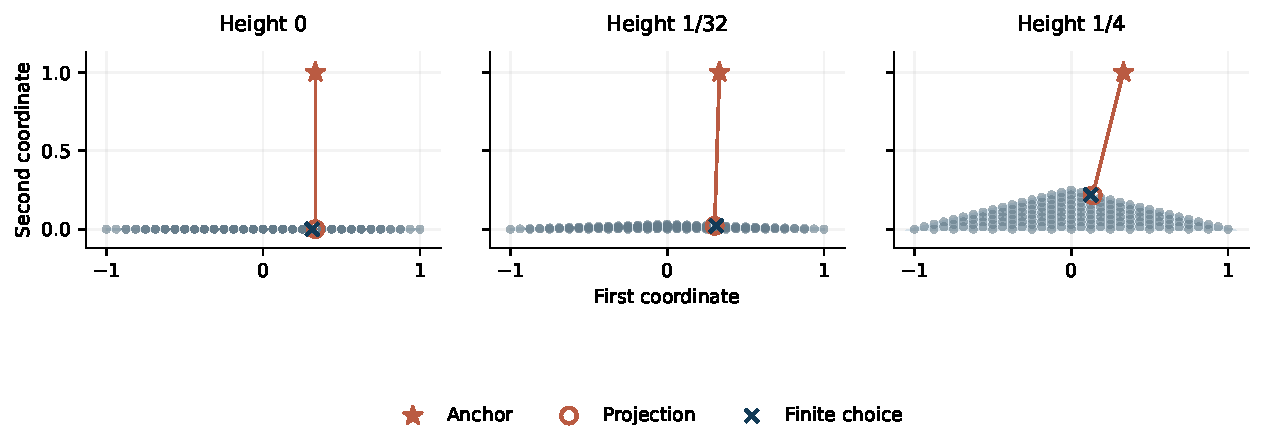
\includegraphics[width=\textwidth]{figures/convex_projection.pdf}
\caption{The same finite-cloud construction for a segment and two thin triangles, with anchor $(1/3,1)$. Gray points use rational simplex weights of denominator sixteen. The finite choice approaches the unique Euclidean projection without testing affine rank. Exact fractions determine the selected points; floating-point coordinates are used only for this illustration.}
\end{figure}

\subsection{Two boundaries that the theorem does not remove}

\paragraph{Hausdorff coherence alone does not stabilize nearest points.}
For \(n\geq1\), let
\[
 S_n=\{-1,\,1+(-1)^n2^{-n}\}\subset\mathbb Q,
 \qquad z=0.
\]
The clouds satisfy \(H_\infty(S_n,S_m)\leq r_n+r_m\).
Their exact nearest point is uniquely \(-1\) for even \(n\), and
uniquely \(1-2^{-n}\) for odd \(n\).  Thus the independently selected
minimizers do not form a Cauchy sequence.  This example involves no tie
ambiguity.  The missing hypothesis is asymptotic midpoint closure: the
limit cloud is the nonconvex set \(\{-1,1\}\).

\paragraph{An equation does not automatically provide a Hausdorff name.}
For a real coefficient \(a\), consider the nonempty compact convex set
\[
 K_a=\{x\in[-1,1]: ax=0\}.
\]
If \(a=0\), then \(P_{K_a}(1)=1\); if \(a\ne0\), then
\(P_{K_a}(1)=0\).  The set-valued input jumps at zero, and so does this
projection.  A finite-observation algorithm cannot produce this projection
uniformly from an arbitrary Cauchy name of \(a\): an observation consistent
with zero is also consistent with a sufficiently small nonzero rational.
Convexity does not remove the need to supply or derive a Hausdorff
presentation of the solution set.  For exact rational \(a\), equality is
decidable and this particular obstruction disappears; the two input
representations must not be conflated.

\subsection{Arithmetic proof audit and Lean completion obligations}

Every executable step uses finite lists, positive-denominator rational
arithmetic, bounded minima, bounded maxima, coordinate sums, or an explicit
dyadic schedule.  Dimension and vertex count may be numerical inputs.
To express the construction in the repository's object theory, encode a
rational as a signed numerator and positive natural denominator; encode a
point and a cloud by the existing sequence programs.  Comparisons are
cross-multiplied integer inequalities.  The guard that denominators are
positive is retained at every division and floor operation.

The essential induction invariants are as follows.
\begin{enumerate}
\item During a finite minimum scan, the saved index is below the processed
      prefix length and its squared-distance score is at most every score
      in that prefix.  The bounded universal comparison is represented by
      the existing Boolean-fold predicate.
\item During a coordinate sum, the partial difference of the two squared
      distances is bounded by \(4B\) times the processed coordinate count
      times the prescribed maximum-norm error.
\item During simplex rounding, the partial sum of floor values is at most
      \(D\), and the accumulated weight error is below the processed
      count divided by \(D\).  The last coordinate is explicitly the
      remaining weight.
\item During enumeration of weight codes, the retained list contains
      exactly the processed tuples with nonnegative entries and sum \(D\).
\end{enumerate}
Each invariant becomes a quantifier-free equation or inequality after
Booleanizing bounded comparisons.  Arbitrarily large numerical loops do
not introduce stronger induction.  Conversely, an abstract Lean proof
using real compactness is not a substitute for these arithmetic
derivations.

The complete Lean path is concrete:
\begin{enumerate}
\item Reuse finite least-argmin, rational arrays, Hausdorff witnesses, and
      bounded reflection from the existing \texttt{Derivations} project.
      Define \texttt{sqDist}, \texttt{cloudMidpointDefect}, and the
      rational \texttt{pick} program.
\item Prove the coordinate polynomial identity and the Lipschitz estimate
      in object arithmetic.  Export the finite comparison theorem as
      a theorem of the form \texttt{Gamma |- [PRAAx] cloudPairBound},
      keeping the cloud hypotheses inside the object formula.
\item Compose that theorem with the existing dyadic-order and
      regular-name modules to prove \eqref{eq:cloud-name}.  The essential
      proof term consumes pairwise finite contracts and performs no
      induction on the unbounded statement ``all later stages are close.''
\item Implement and prove the simplex rounding producer, then specialize
      the generic cloud theorem to \eqref{eq:hull-cloud}.  Bounded
      enumeration has the explicit cap \((D_n+1)^m\).
\item Export represented membership and the minimum-property comparison
      using finite covers and rational slack removal.  Finally prove an
      ordinary Lean semantic interpretation identifying the represented
      point with Euclidean projection.
\end{enumerate}
The present section supplies full human proofs of the finite estimates and
the producer.  The object-language and semantic Lean endpoints are
formalization targets unless a separate build record explicitly marks
them checked.  The included exact-rational program exercises the actual
rounding, finite minimization, and cross-cloud inequality; those executions
validate the implementation examples, not the universal theorem.

\section{A concrete Lean route, and its present status}
\label{sec:lean-route}

The relevant target judgment in the inspected repository is
\begin{center}
\texttt{Prf PRAAx \(\Gamma\) \(\varphi\)},
\end{center}
where \texttt{PTm n} is the syntax of primitive-recursive terms and
\texttt{Fm PTm n} is the syntax of formulas in a common finite scope.
This target must be kept distinct from a theorem about Lean's natural
numbers, rationals, reals, or matrices.  The existing bridge translates
ordinary ConciseIPRA proofs to the Foundation presentation of ordinary
iPRA; the bridge does not convert arbitrary host-level mathematics into
object-theory proofs.

\paragraph{Verification status.}
All repository APIs discussed here were read at revision
\path{3ee850b4c2d650cf01263823fd5415963747c5d0}.
That revision requests Lean \texttt{v4.32.0}.
No Lean executable was available in the preparation environment.
The new Lean source is therefore an \emph{unelaborated formalization
outline}, including a complete proposed proof of the finite cancellation
lemma below.  No new kernel-checked Lean theorem is claimed.
The three runtime norm targets are definitions of remaining obligations,
not admitted theorems.  The absence of an admitted-proof command in those
files is not evidence that the obligations have been discharged.

\subsection{An object-theory lemma with an explicit certificate}

The repository represents an integer term by two natural terms
\(u^+,u^-\), with intended value \(u^+-u^-\).
Its integer comparison \texttt{zle u v} expands to the natural comparison
\(u^++v^-\leq v^++u^-\).
The module \texttt{Core/IntOrder.lean} associates the natural slack
\[
 s(u,v)=(v^++u^-)\mathbin{\dot-}(u^++v^-)
\]
with a proof of this comparison.  Here \(\dot-\) is truncated subtraction.
Thus a signed comparison is usable through an equality with an explicit
nonnegative witness, without deciding the sign of an arbitrary real.

Suppose signed numerators \(A,B,C\) and natural terms \(w,P,e_L,e_R\)
satisfy
\[
 A\leq C+e_L,\qquad B\leq C+e_R,\qquad
 2wC+P\leq w(A+B).
\]
Let their respective slacks be \(s_1,s_2,s_3\).  The whole argument is
the polynomial identity
\[
 w(e_L+e_R)=P+s_3+w(s_1+s_2).
\]
Its right-hand remainder is a natural term, so it proves
\(P\leq w(e_L+e_R)\) in iPRA.
The file \texttt{MidpointCancellation.lean} implements this certificate
using the existing \texttt{zle\_toZ}, \texttt{le\_of\_eq\_add}, and
\texttt{deriveNat} interfaces.  The latter interface reflects a proved
identity in the ring of provable term-equivalence classes back to an
object equation.  It is not reflection from arbitrary truth in the
standard model.

For the cloud theorem, use
\[
 A=2F_z(x),\quad B=2F_z(y),\quad
 C=2F_z((x+y)/2),\quad w=1,\quad P=\|x-y\|_2^2.
\]
The parallelogram identity supplies the third premise.  The two repaired
midpoints supply the first two with
\[
 e_L=L(2\eta_S+h)+2\epsilon_S,\qquad
 e_R=L(2\eta_T+h)+2\epsilon_T.
\]
The resulting object inequality has the exact constant
\[
 \|x-y\|_2^2\leq
 2L(\eta_S+\eta_T+h)+2(\epsilon_S+\epsilon_T).
\]
All rational quantities must first be placed on a common positive
denominator.  The source gives the integral cancellation step; rational
scaling and the geometric hypotheses remain explicit adapter obligations.
The identity itself was independently expanded to zero with exact
symbolic arithmetic.  That check does not constitute Lean elaboration.

\subsection{The finite-cloud implementation}

The dimension, cloud lengths, point coordinates, precision indices, and
error bounds are numerical inputs.  Fix the finite-list and rational
codecs once.  A vector is a numerical list of signed rational coordinate
codes; a cloud is a nonempty numerical list of vectors.  The assertions
of a box bound, sup-norm proximity, Hausdorff proximity, approximate
midpoint closure, and approximate minimality are bounded formulas over
these lists.  Their Boolean translations, rather than the displayed
quantified formulas themselves, are used as induction invariants.

The primitive-recursive selector chooses the least cost-minimizing
index.  The repository already supplies
\texttt{ApproximateWitness.argmin}, its range and attainment theorem,
and \texttt{argmin\_minimal}.  All finitely many costs can be converted
to natural numerators on a common positive denominator.  The selector
therefore compares exact integers; no real comparison is hidden in it.
The actual nearest-neighbor and Hausdorff scans in
\texttt{FiniteHausdorff.lean} can similarly be reused after proving the
chosen vector metric and scaling adapter.

There are four new geometric verification loops.  First, accumulate the
cost over coordinates.  The invariant says that the current accumulator
equals the sum of the first \(i\) squared differences.  Second, prove
the Lipschitz estimate by accumulating the first \(i\) coordinate
estimates, with bound \(4iBh\).  Third, accumulate the coordinatewise
parallelogram identities.  Fourth, apply the bounded midpoint and
Hausdorff witnesses and the argmin theorem to obtain the two comparisons
used above.  All loop lengths are displayed numerical bounds; even a
cubic exhaustive midpoint scan is primitive recursive.

The regular-name theorem then contains only finite comparisons at two
independent precision indices and the explicit precision schedule.
The usual interpretation as a completed real vector belongs to the
external semantic explanation.  No completion, compactness, or infinite
choice axiom is added to the arithmetic theory.

\subsection{The runtime norm targets}

The source \texttt{GaussianPolynomialMonicNorm.lean} already computes
an actual polynomial-valued multiplication matrix and its determinant.
Its inputs \(F,G,m,a,c\) are numerical: \(m\) is not a host-level matrix
dimension.  The stored norm has coarse degree cap
\[
 m\bigl(a+(m-1)c\bigr).
\]
The inspected implementation proves coefficient and evaluation formulas
and binds the actual returned matrix to the source curve equations.
It explicitly leaves norm nonvanishing, sharp degree, the runtime
matrix-kernel implication, fiber multiplicity, and the general coded-field
adapter as further obligations.

The coefficient convention matters.  The array \(F\) stores only the
lower coefficients of a monic polynomial in \(Y\), in descending
\(Y\)-order.  Each row is itself a descending coefficient list in
\(X\).  Row \(i<m\), slot \(j\leq c\), therefore corresponds to
\(X^{c-j}Y^{m-1-i}\).  The shape predicate fixes each used row's width;
it does not require raw rational codes to be canonical.  Weighted support
is consequently tested after coefficient normalization.

The file \texttt{RuntimeNormTargets.lean} defines the exact closed
object-theory target saying that a common zero of the original monic
polynomial and \(G\) is a zero of the actual computed norm.  This target
does not accept a determinant-kernel theorem as an input assumption.
The existing \texttt{returned\_zero\_action} gives every coordinate of
the relevant left-kernel equation.  The remaining finite determinant
argument must use the actual numerical determinant and the fact that
the first evaluation-vector coordinate is one.

For the weighted-degree target, use integer weights
\(w_X\geq1\), \(w_Y\geq0\).  The finite support requirements are
\[
 w_X(c-j)+w_Y(m-1-i)\leq mw_Y
\]
for nonzero lower coefficients of \(F\), and the analogous inequality
with cap \(D\) for \(G\).  The conclusion states that the actual norm's
leading slots above \(\lfloor mD/w_X\rfloor\) vanish.  It is a support
statement, not a claim that the already allocated buffer gets shorter.

The required induction invariant for the \(j\)-th companion iterate is
\[
 w_X\deg_X h_r+w_Yr\leq D+w_Yj,
\]
for each nonzero coefficient polynomial \(h_r(X)\) of \(Y^r\).
Use bounded coefficient convolution and the monic relation to prove one
step.  Apply quantifier-free induction to the Booleanized support
predicate over the actual column loop.  In each determinant term the
row-weight sum equals the column-weight sum because the numeric word
encodes a permutation.  The \(w_Y\)-contributions cancel; hence every
term has \(X\)-degree at most \(\lfloor mD/w_X\rfloor\).
A second bounded induction over the permutation scan proves the leading
zero coefficients of the stored determinant.

The repository's fixed-size determinant laws give useful mathematical
templates.  They are not already the numerical-dimension theorem just
described.  The runtime scan, its coverage and uniqueness, and an actual
adjacent-column alternation implementation are available and should be
the starting point.  The archive's formalization plan lists the exact
source paths and the remaining steps, including the separate
nonvanishing and fiber-multiplicity arguments.

\subsection{A finite-place certificate for nonvanishing}

The third target, \texttt{LocalNewtonNormTarget}, uses the existing
numeric translation program
\texttt{GaussianRationalTranslation.translated}.
For a stored polynomial of degree cap \(C\), its entry at \(C-i\)
is the coefficient of \(T^i\) in \(P(a+T)\).
The predicate \texttt{exactOrder} requires a specified nonzero leading
coefficient and zero coefficients at every smaller index.
All these checks are finite; no formal-series object or infinity-valued
valuation is a term of the arithmetic language.

The local certificate for
\(F=Y^m+\sum_{j<m} f_j(X)Y^j\) gives \(e\geq1\),
\(\gcd(m,e)=1\), and \(c_0\ne0\), such that \(f_0(a+T)\)
has order \(e\) and leading coefficient \(-c_0\).
For \(0<j<m\), every coefficient of \(T^i\) with
\(mi+ej\leq me\) vanishes.  This finite support condition handles a
zero coefficient polynomial without a special valuation convention.
For reduced \(G\), a second certificate identifies a nonzero coefficient
\(bT^vY^k\), \(k<m\), at minimal weight \(s=mv+ek\).
The coprimality condition makes the minimal pair unique.

The proposed endpoint asserts that the actual computed norm has exact
order \(s\) at \(a\), with leading coefficient
\[
 b^m\bigl((-1)^{m-1}c_0\bigr)^k.
\]
It also gives the independent global degree bound under the global
weighted-support hypotheses.  Both conclusions refer to the original
numeric norm program; the desired nonvanishing statement is not an
input premise.

For formalization, one need not introduce Puiseux roots.  At initial
weight the reduction relation is \(Y^m=c_0T^e\).  In multiplication
column \(j\), the initial monomial goes to row
\((k+j)\bmod m\), with coefficient
\(b c_0^{\lfloor(k+j)/m\rfloor}\) and \(T\)-exponent
\(v+e\lfloor(k+j)/m\rfloor\).
This row pattern is a permutation.  Its product has order \(mv+ek\),
and its cyclic-shift sign is \((-1)^{(m-1)k}\).
For any other contribution, the strict weight excess survives after the
row and column weights cancel.  Finite support induction, the actual
permutation codec, and coefficient convolution therefore provide a direct
path to the displayed coefficient formula.  Proving these connections in
Lean remains work identified by the target, not work reported as checked.

\subsection{Formalizing the polynomial-division nonvanishing certificate}
\label{sec:squarefree-lean}

The squarefree norm theorem admits a direct numerical formalization that
does not construct roots or formal branches.  Its input is a list of
exact coefficient codes for \(g,h,A_0,\ldots,A_{m-1}\), numerical
\(m,e\geq1\), and finite certificates
\[
 f=g^e h,\qquad \alpha g+\beta h=1,\qquad
 Ug+Vg'=1,\qquad \gcd(m,e)=1,\qquad\deg g\geq1.
\]
Coefficient equality and zero tests mean equality after normalization,
checked over an explicitly padded finite list.  The theorem to be
exported concerns the existing numeric norm program for \(Y^m-f\).
The ordinary Mathlib goals in the archive are semantic targets; they do
not themselves have the object-theory type \texttt{Prf PRAAx}.
For the existing constructor, store \(m\) descending \(Y\)-rows for
\(F\), all zero except the last row \(-f\), and store
\(A_{m-1},\ldots,A_0\) for \(G\).  Pad each row to a common
displayed \(X\)-degree cap.  These finite constructions discharge the
existing row-shape guards.

\paragraph{The producer and its bounded invariant.}
General long division over the coefficient field can be implemented in
\(\operatorname{degcap}(A)+1\) steps; an arbitrary nonzero leading coefficient is
handled by exact rational inversion.  Repeating division by \(g\) uses
another loop with the same cap, freezing at the first nonzero remainder.
For nonzero \(A\), the active-state invariant is
\[
 A=g^aB,\qquad B\ne0,\qquad
 \deg B+a\deg g=\deg A.
\]
This proves termination because \(\deg g\geq1\).
A separate zero flag handles \(A=0\); no infinity-valued order is
encoded.  All degrees are bounded scans of normalized coefficients.
The resulting factors \(A_j=g^{a_j}B_j\) determine the least weight
\(s=ma_k+ek\), using a finite scan over nonzero indices.

\paragraph{The actual determinant identity.}
In column \(c\), reduction of \(A_jY^{j+c}\) uses
\(j+c=r+m\delta\), with \(r<m\) and \(\delta\in\{0,1\}\).
Its matrix entry is \(A_jf^\delta\).  For each numerical permutation
word, summing this identity gives
\(\sum_c j_c=m\sum_c\delta_c\).
Thus its \(g\)-exponent \(E\) satisfies
\[
 mE=\sum_c(ma_{j_c}+ej_c)\geq ms.
\]
Equality forces every \(j_c=k\), so the unique minimal term is the
cyclic row permutation \(c\mapsto(k+c)\bmod m\).  Its carries sum to
\(k\), and its sign is \((-1)^{k(m-1)}\).
All other nonzero terms have \(E\geq s+1\).  The remainder polynomial
\(Q\) is therefore constructed directly by summing their signed
products with exponents \(E-s-1\).  This proves the finite certificate
\[
 N=g^s\left((-1)^{k(m-1)}B_k^m h^k+gQ\right).
\]
The existing permutation scan has horizon \(m^m\).
Prefix identities for products and sums, together with the actual
coefficient Leibniz theorem, provide the quantifier-free induction route.

\paragraph{Reducedness by explicit Bezout identities.}
To prove \(g\mid B^r\Rightarrow g\mid B\), compute
\(D=\gcd(g,B)\), write \(g=DC\), \(B=DE\), and retain an extended
gcd certificate.  It yields a Bezout identity for \(C,E\).
Substituting \(g=DC\) into \(Ug+Vg'=1\) gives
\[
 C(UD+VD')+D(VC')=1.
\]
Multiplying these two identities gives \(HC+JB=1\).
If \(C\mid B^r\), the finite identity
\[
 1-(JB)^r=HC\sum_{i<r}(JB)^i
\]
exhibits an inverse for \(C\).  Consequently \(g\mid B\).
The zero-polynomial case is immediate; all other cancellations have
explicit nonzero factors.  This is a finite polynomial-gcd proof of the
required reduced quotient property, with no factorization step.

Because \(B_k\) has nonzero remainder and \(h\) is invertible modulo
\(g\), the parenthesized factor in the norm identity has nonzero
remainder.  It follows that the norm is nonzero and its exact
\(g\)-divisibility order is \(s\).  A bounded scan of its actual output
buffer then returns a nonzero coefficient: if the scan failed, every
coefficient would be zero, contradicting the residue calculation.

For squarefree nonconstant rational \(f\), take \(g=f,e=1,h=1\).
The extended gcd of \(f,f'\) supplies the reducedness certificate.
The new Lean obligations are the general polynomial-division and gcd
loops, their invariants, the runtime carry/sign proof, and binding the
coefficient identity to the existing norm output.  Existing synthetic
division and monic reduction are useful templates; this report does not
assert that a general-divisor API is already available.
The attached source and roadmap remain uncompiled formalization outlines.

\section{What the framework resolves, and where the boundary moves}
\label{sec:limits}

\subsection{A broader view of finite algebraic intermediates}

The squarefree norm proof illustrates a reusable replacement for field extensions chosen by existence arguments. Construct a finite algebra whose entries are explicit coefficient vectors. Prove the operations and the exact property used by the argument: an element may have a supplied inverse; a quotient may be reduced; a matrix may have a supplied right inverse. Carry that property as a proved invariant. A field structure is unnecessary when the calculation only uses ring identities and a few certified units.

This distinction matters because a nonzero element in a finite algebra need not be invertible. In $\Q[u]/(u^2-1)$, the element $u-1$ is a nonzero zero divisor. Its square is still nonzero, which is the property the norm argument needs. Replacing this algebra by an unspecified field would hide a branch choice; treating every nonzero element as invertible would make the proof false. The certificate discipline identifies a weaker sufficient algebraic structure and verifies it directly.

The same strategy can be used for symmetric polynomial observations, quotient-ring identities, finite multiplication matrices and algebraic function calculations that do not require naming an individual branch. Whenever division occurs, replace it by an explicit unit witness and an equation $uv=1$. The output may then be a polynomial identity or a scalar nonvanishing statement over the original field. One must still prove any final descent step; a statement about a chosen quotient value is not automatically a statement about every possible root.

\subsection{Canonical observations of nonunique solution sets}

The convex selector is a second broadly reusable operation. Original witnesses need not be unique. What must be unique, quantitatively, is the answer to the specified query: nearest to a fixed anchor. Squared-distance minimization supplies this property from midpoint convexity. The finite comparison theorem then transforms geometric structure into a cross-query modulus.

Thus two common obstacles have different remedies. Algebraic branch selection can sometimes be removed by keeping an entire finite algebra or root aggregate. Nonunique geometric witnesses can sometimes be made canonical by a strictly convex query. Neither remedy applies universally. A disconnected two-point set defeats the projection coherence argument; discontinuous solution-set formation defeats the Hausdorff input requirement.

\subsection{A finite cover search is not its existence theorem}

There is a useful exact reduction for the Diophantine program. Suppose $N$ supplied vectors in $K^n$ admit a cover by $C$ proper linear subspaces. For each subspace, replace it by the span of the listed vectors assigned to it. Bounded Gaussian elimination chooses a basis of at most $n-1$ of those vectors. Consequently one may search for the cover among spans of at most $n-1$ input vectors.

Allowing a zero-vector sentinel, at most $(N+1)^{n-1}$ ordered candidate generator lists are needed for one subspace, and at most
\[
 (N+1)^{C(n-1)}
\]
for $C$ subspaces. Exact row elimination checks properness and membership. Thus the existence of a cover of this supplied list implies success of a bounded primitive recursive search. If $n=1$, every proper linear subspace is zero, and the same formula has exponent zero; the degenerate case is explicit.

The missing input is the mathematical proof that every relevant point list has such a cover with the stated numerical $C$. The search does not prove that fact. In the Siegel setting, producing or proving the required covers can encode the difficult approximation theorem. The norm result now discharges the zero-count consequence for a larger curve class, but does not discharge the cover theorem itself \cite{repo-siegel}.

\subsection{Cardinality, height, and complete enumeration}

A bound of $M$ on the number of solutions says that every list of $M+1$ distinct candidates contains a failure. It does not say where the solutions lie. Even a uniform cardinality bound of one cannot generally supply a height bound or a decision that the unique possible solution exists.

Here is an exact obstruction. Let $H(e,t)$ be the primitive recursive predicate that the machine coded by $e$ halts for the first time at step $t$. For each $e$, at most one $t$ satisfies $H(e,t)$. If an algorithm could uniformly produce a complete finite list of all such $t$, it could decide whether the machine halts by testing whether that list is empty. If a total computable cutoff $B(e)$ satisfied $H(e,t)\Rightarrow t\le B(e)$, bounded simulation would likewise decide halting. Thus finite-list completeness and cutoffs require information stronger than a cardinality estimate. This is a statement about general predicates, not a claim that a particular Diophantine curve has an uncomputable height bound.

For a concrete polynomial problem, a height-to-code adapter also needs proof. If rational coordinates have reduced numerators of absolute value at most $H$ and denominators between one and $H$, there is an explicit finite grid of candidate codes. But the theorem supplying such an $H$ is a separate input. The current improvement gives finite common-zero and subspace-fiber bounds; it is not a general effective Faltings theorem \cite{repo-faltings}.

\subsection{A regular approximation does not decide equality}

A fast Cauchy name supplies approximations with explicit error. It cannot in general decide whether its limit is zero. Indeed, any fixed finite set of observations consistent with zero is also consistent with a sufficiently small nonzero rational. An algorithm deciding zero would have to distinguish these from that same finite information. Inverse operations therefore need positive apartness data, such as a rational lower bound on absolute value. Matrix rank or the degree of a polynomial with arbitrary Cauchy coefficients likewise needs a suitable separation witness or a weaker output representation.

Our exact algebra uses rational or other exactly coded coefficients. Our convex-hull producer, by contrast, tolerates coincident and affinely dependent named vertices because it performs no real-equality or rank test. The representation choice is part of the theorem, not an implementation footnote.

\subsection{How to reuse the discipline across the portfolio}

\begin{longtable}{@{}P{0.22\textwidth}P{0.33\textwidth}P{0.39\textwidth}@{}}
\toprule
Mathematical topic & Appropriate finite interface & Substantive producer to prove\\
\midrule
\endhead
Algebraic equations & Exact coefficient buffers; multiplication matrices; root-support observations & Monic reduction, guarded nonvanishing, or a certified finite root approximation. Selecting a branch is a separate demand.\\[4pt]
Analytic functions & Rational evaluations with domains, bounds and moduli & Tail estimates and evaluators with actual precision schedules. A formal power series alone is not a convergence proof.\\[4pt]
Convex geometry & Finite Hausdorff clouds, midpoint defect and coordinate box & Cloud generation from the original description. Named vertices are handled here; arbitrary constraints need their own stability data.\\[4pt]
Linear algebra & Exact runtime matrices or approximation matrices with gaps & Pivot witnesses for exact fields; quantitative separation for spectral subspaces when required.\\[4pt]
Diophantine geometry & Finite point lists, weighted evaluations, annihilator certificates & Cover existence and height bounds. This report broadens the zero-count component.\\[4pt]
Topology & Finite triangulations, covers and compatible local data & Explicit mesh or subdivision bounds and the finite combinatorial theorem. An arbitrary infinite branch is not automatically available.\\[4pt]
Probability & Finite outcome tables, rational weights and event bits & Quantitative tails or exceptional-set bounds for any limiting assertion; finite inequalities alone do not choose an almost-sure witness.\\[4pt]
Category-theoretic structure & Finite tables or fixed schematic operations with congruence laws & Actual universal-object constructions and bounded equality laws in the chosen presentation.\\
\bottomrule
\end{longtable}

The framework helps by making these producers composable and by showing where stronger-looking mathematical objects can be replaced by finite ones. It does not erase a missing analytic estimate, an unbounded compactness principle, or an unproved Diophantine bound. The practical next step is to implement the new producer lemmas against the existing numerical arithmetic, so their actual closed sentences become reusable dependencies in the same way as the already checked finite-demand machinery.

\section{Artifacts, reproducibility, and exact proof status}
\label{sec:artifacts}

\subsection{Contents of the archive}

The main source is \path{paper/report.tex}, with section files and this compiled PDF. The \path{code/} directory contains exact-arithmetic reference implementations for polynomial norm certificates and convex clouds. The \path{lean/} directory contains the proposed midpoint-cancellation proof, explicit runtime norm targets, the pinned toolchain identifier, a checking script and the formalization roadmap. The \path{research/} directory records the source audit, inspected predecessor relationships and independent mathematical checks. The \path{validation/} directory records executed finite checks.

The selected upstream source snapshots are evidence for the audit, not a complete self-contained Lean dependency closure. To elaborate the new candidate sources, use the pinned ProveIt checkout and its declared package dependencies. The checking script verifies the checkout's commit before invoking the upstream build. No new repository-wide build was performed for this report.

\subsection{Validation that was actually run}

The norm program constructs multiplication matrices by actual monic remainder, computes their determinants by a literal signed permutation expansion, and compares them with an independent resultant calculation. It checks:
\begin{itemize}
\item 54 mixed local-Newton cases, including translated rational centers, varying local orders, and the predicted nonzero initial coefficient;
\item 41 compressed leading-coefficient cases, including successful certificates and exact leading cancellation;
\item 80 squarefree finite-algebra cases, including quotient rings with zero divisors, against the local formal-root version of the argument;
\item 29 separate polynomial-division-order certificates over $\Q$, $\mathbb F_2$ and $\mathbb F_3$, including characteristic dividing $m$, positive division order and nonzero zero-divisor residues;
\item explicit fiber multiplicity and zero-norm counterexamples.
\end{itemize}

The convex-cloud program uses \code{fractions.Fraction} throughout. It checked 4,474 cloud/anchor combinations against both finite comparison inequalities, 3,101 simplex-rounding cases, 3,101 midpoint certificates, and 1,127 cross-cloud transfer certificates. It includes the alternating nonconvex counterexample and 12 exact projection examples through affine rank collapse.

These are finite execution checks. The universal results rest on the proofs in this report. In particular, checking many resultants does not prove the numerical-dimension norm theorem; checking a proposed Lean statement as a definition would not prove it either.

\subsection{Formalization ledger}

\begin{longtable}{@{}P{0.33\textwidth}P{0.27\textwidth}P{0.34\textwidth}@{}}
\toprule
Result & Present evidence & Further Lean work\\
\midrule
\endhead
Global norm support and mixed local order & Full human proofs, coefficient invariants, exact examples & Actual runtime support and rescaling/word identities.\\[4pt]
Reduced quotient and polynomial-division-order norm & Full factorization-free human proof; exact finite-field checks & Runtime polynomial Euclid, divisibility witness and determinant carry export.\\[4pt]
Compressed leading coefficient & Full block decomposition proof; exact comparisons & Basis permutation and block determinant for the actual codec.\\[4pt]
Common-zero and subspace caps & Full human proofs; source-specific integration plan & Runtime multiplicativity/fiber factors and nonzero annihilator producer.\\[4pt]
Finite midpoint cancellation & Explicit proposed \code{Prf PRAAx} proof; symbolic slack identity & Elaborate the candidate and resolve any API issues.\\[4pt]
Convex selector and hull-cloud producer & Full human proofs and exact rational tests & Rational scaling adapters, coordinate identities, actual returned-name contract.\\[4pt]
Projection in completed $\R^d$ & External semantic argument & A separate Lean semantic theorem, distinguished from object arithmetic.\\
\bottomrule
\end{longtable}

The new Lean sources are unelaborated: no Lean executable or compiled dependency cache was available in this environment. They are labeled accordingly. There are no claims that the new norm theorem, canonical selector, or their object-language endpoints have already been kernel-checked. Existing upstream checked status is reported from the exact inspected source revision.

\subsection{Recommended implementation order}

The shortest useful algebraic path begins with the special superelliptic matrix, not the full mixed-curve machinery. Prove the coefficient support budget and the determinant carry identity, then the repeated-division and reducedness lemmas. This yields the new nonzero-norm endpoint. In parallel, use the existing fiber grouping and completed-matrix inverse to obtain determinant fiber divisibility; this gives the finite zero count. Finally add the runtime annihilator producer for the proper-subspace corollary. The mixed local-rescaling theorem and compressed leading determinant can be independent later modules.

For the selector, first elaborate the short integral cancellation lemma. Then connect the rational squared-distance code and the finite nearest/midpoint witnesses to it. The dyadic reindexing theorem needs only the resulting pairwise estimate. The convex-hull input producer has a direct rounding proof and no rank analysis. Only after these arithmetic endpoints are checked should a completed-real interpretation be exported.

\begin{thebibliography}{99}
\small
\bibitem{repo-audit}
Vladimir Reshetnikov, ProveIt, \emph{Finite-demand source-claim audit}, pinned revision \texttt{\pin}, 19 November 2026.
\url{https://github.com/VladimirReshetnikov/ProveIt/blob/3ee850b4c2d650cf01263823fd5415963747c5d0/Logic/PrimitiveRecursiveArithmetic/Derivations/FINITE-DEMAND-CLAIMS.md}.

\bibitem{repo-derivations}
ProveIt, \emph{iPRA Derivations: module and source inventory}, same pinned revision.
\url{https://github.com/VladimirReshetnikov/ProveIt/blob/3ee850b4c2d650cf01263823fd5415963747c5d0/Logic/PrimitiveRecursiveArithmetic/Derivations/README.md}.

\bibitem{repo-concise}
ProveIt, \emph{ConciseIPRA}, ordinary theory, native theory, and their formal translations, same pinned revision.
\url{https://github.com/VladimirReshetnikov/ProveIt/tree/3ee850b4c2d650cf01263823fd5415963747c5d0/Logic/PrimitiveRecursiveArithmetic/ConciseIPRA}.

\bibitem{repo-norm}
ProveIt research packet \emph{ipra\_finite\_demand}, section ``Automatic norm certificates and sharp finite zero counts,'' same pinned revision.
\url{https://github.com/VladimirReshetnikov/ProveIt/blob/3ee850b4c2d650cf01263823fd5415963747c5d0/Logic/PrimitiveRecursiveArithmetic/docs/proofs/foundations/ipra_finite_demand/sections/05_norm_certificates.tex}.

\bibitem{repo-coherent}
ProveIt research packet \emph{ipra\_coherent\_methods\_2026-11-15}, norm section, including ``A broader finite certificate when coprimality fails,'' same pinned revision.
\url{https://github.com/VladimirReshetnikov/ProveIt/blob/3ee850b4c2d650cf01263823fd5415963747c5d0/Logic/PrimitiveRecursiveArithmetic/docs/proofs/foundations/ipra_coherent_methods_2026-11-15/paper/sections/05_norms.tex}.

\bibitem{repo-monic-norm}
ProveIt, \emph{GaussianPolynomialMonicNorm.lean}, actual numerical multiplication matrix, norm and returned-field contracts, same pinned revision.
\url{https://github.com/VladimirReshetnikov/ProveIt/blob/3ee850b4c2d650cf01263823fd5415963747c5d0/Logic/PrimitiveRecursiveArithmetic/Derivations/Lean/IPRADerivations/Analysis/GaussianPolynomialMonicNorm.lean}.

\bibitem{repo-strong}
ProveIt, \emph{StrongMinimizer.lean}, same pinned revision.
\url{https://github.com/VladimirReshetnikov/ProveIt/blob/3ee850b4c2d650cf01263823fd5415963747c5d0/Logic/PrimitiveRecursiveArithmetic/Derivations/Lean/IPRADerivations/Foundations/StrongMinimizer.lean}.

\bibitem{repo-siegel}
ProveIt research packet \emph{siegel\_ipra}, general route and its explicit producer obligations, same pinned revision.
\url{https://github.com/VladimirReshetnikov/ProveIt/blob/3ee850b4c2d650cf01263823fd5415963747c5d0/Logic/PrimitiveRecursiveArithmetic/docs/proofs/diophantine-number-theory/siegel_ipra/paper/05_general_route.tex}.

\bibitem{repo-faltings}
ProveIt research packet \emph{faltings\_ipra}, statement of scope and limitations, same pinned revision.
\url{https://github.com/VladimirReshetnikov/ProveIt/blob/3ee850b4c2d650cf01263823fd5415963747c5d0/Logic/PrimitiveRecursiveArithmetic/docs/proofs/diophantine-number-theory/faltings_ipra/README.md}.

\bibitem{kohlenbach-pra}
Ulrich Kohlenbach, ``Things that can and things that can't be done in PRA,'' \emph{Annals of Pure and Applied Logic} 102 (2000), 223--245. Author's manuscript:
\url{https://www2.mathematik.tu-darmstadt.de/~kohlenbach/paper18.pdf}.
Used for context about the sensitivity of conservation and analysis principles, not as an automatic transfer theorem for the present proofs.

\bibitem{leroux-pauly}
St\'ephane Le Roux and Arno Pauly, ``Finite choice, convex choice and finding roots,'' \emph{Logical Methods in Computer Science} 11(4:6), 2015.
\url{https://doi.org/10.2168/LMCS-11(4:6)2015}.
Primary article page: \url{https://lmcs.episciences.org/1607}.
Used for background on represented choice problems; the quantitative cloud estimates here are proved directly.
\end{thebibliography}

\end{document}
